\documentclass[11pt,letterpaper,titlepage]{book}

\pagestyle{headings}

\usepackage{geometry}                
% See geometry.pdf to learn the layout options. There are lots.

\geometry{letterpaper}                   
% or a4paper or a5paper 

\usepackage[parfill]{parskip}
% Activate to begin paragraphs with an empty line rather than an indent

%\usepackage{hyperref}		
% create clickable links in the document

%\usepackage{graphicx}
\usepackage{amssymb,amsmath}

%\usepackage{epstopdf}

\usepackage{textcomp} 
% for degree C

\usepackage{rotating} 
% sidewaystable

\usepackage{array} 
% table centering

\usepackage[small,bf]{caption} 
% makes captions look nicer 

\usepackage{placeins} 
% this is required for \FloatBarrier, 
% which is used to prevent figures from being placed across section breaks.

\usepackage{algorithmic}
% for if .. then logic

\usepackage{makeidx}
\makeindex

\DeclareGraphicsRule{.tif}{png}{.png}{`convert #1 `dirname #1`/`basename #1 .tif`.png}

\title{Open Stent Design}

\author{Craig Bonsignore\\
  NDC\\
  47533 Westinghouse Drive\\
  Fremont, CA, 94566\\
  \texttt{craig.bonsignore@nitinol.com}}


%\date{}  % Activate to display a given date or no date

% \numberwithin{equation}{section} 
% format equation numbers (chapter.section.number) rather than (chapter.number)

\begin{document}

\maketitle

\copyright2011 Nitinol Devices \& Components, Inc. Some rights reserved.

This work is licensed under the Creative Commons Attribution-Share Alike 3.0
United States License. To view a copy of this license, visit
http://creativecommons.org/licenses/by-sa/3.0/us/ or send a letter to Creative
Commons, 171 Second Street, Suite 300, San Francisco, California, 94105, USA.

This document is distributed in the hope that it will be useful, but WITHOUT ANY
WARRANTY; without even the implied warranty of MERCHANTABILITY or FITNESS FOR A
PARTICULAR PURPOSE.

% \begin{abstract}
% My abstract goes here. Hello, I'm an abstract. This is a small change.
% \end{abstract}

\tableofcontents{}
\newpage

\addcontentsline{toc}{chapter}{Introduction}
\chapter*{Introduction}

\section*{Why Open Stent Design?}

This project is intended to bring the collaborative principles of open source to
the typically closed and proprietary world of medical device development. NDC has
a long history pioneering development of Nitinol stents and similar components,
and has also been a leading publisher and educator in the field. Contributing to the
open source and creative commons movements is a natural evolution of our
commitment to Nitinol education. It is our hope that providing these tools and
resources in an unlimited way to the community of medical device developers, as
well as academic researchers, reviewers, and others, we will inspire a new
generation of designers with ideas that will advance the state of the art, and
the practice of medicine.

\section*{Thoughts on Intellectual Property}

It is nearly impossible to separate commercial medical device development from
intellectual property. Bringing a medical component to market, especially in the
case of an implant, is an exceptionally expensive affair. The level of upfront
investment is high, the road is long, the outcome is uncertain. If the
constellations align, the rewards are great. Consequently, any investor (whether a venture
capitalist, or the R\&D department of a large corporation) considering
funding a medical device development endeavour is very concerned about intellectual 
property (IP) ownership and rights.  IP is a broad term that includes creative
works that may be protected by trade secrets, copyrights, trade secrets, or
patents. In the case of medical component design, the focus is typically on
patents and the issue for an investor is simple: after I invest my capital in
developing this design, will someone else be able to simply copy my work and
unfairly reap the benefit of my investment? Without patent protection, the
risks to the potential investor may be unacceptably high, and consequently the
investment may not be made, and the invention may never come to fruition.

So in the medical device business, just about everything we do is covered by
patents, patent applications, trade secrets, and/or confidentiality agreements.
The objective of any design is to create something novel and differentiated that can
be protected by patents and distinguished in the marketplace. Companies work
hard to preserve these benefits by enforcing strict practices of secrecy. So the
medical device industry is proprietary by nature; the natural incentives in the
indusrtry promote secrecy and discourage sharing. In this way, the theory goes, 
innovation is enabled by providing the economic rationale for investments in expensive
projects with long development cycles. 

The proprietary nature of the medical device industry creates some
difficulties when those of us inside the industry are motivated to share design guidance, principles,
and techniques: Every realistic example we know about is proprietary!
This manuscript seeks to circumvent this problem by creating a realistic medical
component, the ``Open Stent''  that is completely generic, and using it as an
example to discuss useful techniques and procedures relating to design and
analysis of similar components.

In the microelectronics, software, and entertainment  industries, by contrast,
the development cycle is much shorter, the regulatory barriers are much lower, and intellectual
property flows much more freely. The speed of innovation in these industries
is ferocious. This accelerated culture of collaboration is enabled
by the principles of \emph{open source} development. In this model, creative
individuals contribute their effort to a project, in exchange for a promise: I
will donate my efforts to the commons, and in exchange the community can build
upon my work, and society will enjoy the benefits of our collective efforts.
This approach works quite well in the case of software, where IP is neatly
embodied in lines of code that can be easily exchanged. 

In the medical device industry, there is no direct equivalent of ``lines of
code.'' Instead, there is a constellation of resources, including sketches,
drawings, specifications, protocols, procedures, processes, and so on. In
practice, though, much of this gets reduced to ``lines of code,'' in a
figurative and often literal sense. Design specifications are often created
using computer aided (CAD) systems, detailed in spreadsheets, and analyzed using
sophisticated computer simulations. All of these things share the character of
software code: they neatly capture creative effort, they are readily
portable, and are easily shared and extended.

So this brings us to the purpose of this manuscript. Stents have been around for
quite some time, thousands of stent related patents have been granted, and many
more have been applied for. In IP terms, this means that there is a significant
amount of \emph{prior art} in the field. Because of all the published patents
and other works in the public domain, it is now exceedingly difficult to develop
novel designs in this field. The stent design used throughout this manuscript,
instead, takes the opposite approach: it is intended to be completely generic,
and intentionally \emph{not} novel.

While the stent design itself is quite general, the techniques and resources
that are described here are creative works that have not been previously
published, and (we hope) are useful, practical, and can be extended, expanded
upon, and applied to new, different, and novel designs. Our motivation for this
is simple: we want the medical design community to have the best tools and
resources available for designing Nitinol medical devices. In doing so, the
community benefits, society benefits, and NDC benefits along the way. 

\section*{Thoughts on Licensing}

In the past few years, a variety of standardized licensing strategies have been
developed to aid and encourage efforts such as these. Typically, the 
copyright for creative works such as this manuscript is typically held by the
author. In the era of the printing press, an author assigned his or
her copyrights to a publisher, because only publishers had the means to
duplicate and distribute content to reach a large audience. In the modern internet era, any content can
be made available instantaneously throughout the world, with minimal cost. The
intent of this publication is to reach as wide an audience as possible, and to
make it as easy as possible to apply and adapt the content for new purposes. 

To serve this purpose, this document is offered with a Creative Commons
Attribution-Share Alike 3.0 United States License. A simple explanation of
the license can be found at http://creativecommons.org/licenses/by-sa/3.0/us/,
but it basically means that you are free to share, copy, distribute, and adapt this
work under two simple conditions: 1) any copies or adaptations must provide
attribution to the original author, and 2) any derivitive works must carry the
same freedoms as those afforded by this license. 

\section*{Publication, Attribution and Feedback}

The version of this manuscript that you are currently reading is an unfinished
working draft. We intend to continue to add and edit content, and hope to
incorporate thoughts and feedback from the community. We plan to publish this
through formal channels at some point in the near future, simply because a bound
volume is often more convenient than an electronic version, and futher, it is
helpful to have a more formal means to cite the work in other
publications. The terms of the license require any copies or derivative works to
include a reference to the title and author. Though not strictly required, the
author is quite interested in your thoughts on this work, and any improvements
or adaptations you may make. The online home for this work can be found at
http://nitinoluniversity.com, and we encourage you to visit us there to provide
your feedback, and check for updates or new revisions as they become available.
There you will also find additional resources relating to this work, including
links to the design files, spreadsheets, finite element analysis input files,
and related items.

Now go forth, remix, reuse, recycle. Everybody wins.


\chapter{Basic Elements of Stent Design}

The word \emph{stent} is used to describe any artificial structure that is used
to provide support or scaffolding to a lumen or cavity within the body. The term
is often credited to Charles Stent, a nineteenth century English dentist
\cite{Ring:2001fk}, and came into common use the medical field with
the introduction of the Wallstent, co-invented by Hans I. Wallst\'en in the
1980's \cite{wallsten} \cite{Rousseau:1987fk}. Modern stents are used throughout
the human body, most commonly in arteries of the heart, neck, and lower limbs. Many other stent
applications exist throughout the cardiovascular, pulmonary, and gastrointestinal
systems of the body. Stents are typically fabricated from metals like stainless
steel, cobalt alloys, or nitinol, and some polymer based designs are also being
investigated.

\section{Introduction to Nitinol}

Nitinol, a nearly equiatomic alloy of nickel and titanium, is one of many
materials that is commonly used to fabricate cardiovascular implants such as
stents. Unlike traditional engineering materials like stainless steel and
cobalt alloys, Nitinol exhibits the unusual properties of \emph{shape
memory} and \emph{superelasticity}. These properties are manifestations of a
\emph{phase change} that occurs in the material as it transitions between a
higher temperature \emph{austenite} phase and a lower temperature
\emph{martensite} phase. The mechanical properties of these phases are quite
different, and the transition between the phases creates unusual properties that
are useful for many medical applications.

The temperature at which the phase change occurs, the \emph{transition
temperature} is critically important to the mechanical properties of the
finished component. More specifically, it is the \emph{difference} between the 
transition temperature and the environmental
temperature that dictates performance. This is one of the reasons that Nitinol
works so well in medical applications: the environmental temperature of the
human body is very stable, therefore the mechanical properties of a Nitinol
implant are also stable. 

When the material is substantially below its transition
temperature, it is fully martensitic, and has material characteristics much like
soft lead. It is easily deformed, and will remain deformed, just like any
ordinary material. The unusual properties of Nitinol are demonstrated when
the material is heated above its transition temperature to return to its
austenitic phase. Now, this same material will spontaneously recover to its
original shape, as if it had never been deformed. This demonstrates the
\emph{shape memory} property of nitinol. 

When the material is substantially above its transition temperature, it is fully
austenitic, and has material properties more like steel than lead. It is very
elastic, with much higher stiffness than it had in the marensitic phase, though
lower stiffness than typical stainless steels or other conventional engineering
materials. Unlike typical materials, though, austenitic Nitinol can be deformed
to a very substantial degree, and still recover to its original shape. This is a
demonstration of \emph{superelasticity}, and it is enabled by the stress induced
transformation from austenite to martensite in local regions of high stress. 

For all of these reasons, the transition temperature of a Nitinol component is
of critical importance. It is commonly measured using a \emph{bend free
recovery} technique, wherein the component is cooled until it is fully
martensitic, deformed to a specific shae, then slowly warmed to higher
temeperatures while measuring the recovery to its original shape. Results from a
typical transition temperature test are shown in Figure \ref{fig:af-test}. The
test begins at position 1. When heated, the shape begins to recover at position
2, and completes its recover fully by position 3. Tangent lines are drawn as
indicated to establish $A_s$, the \emph{austenite start} temperature, and the
more commonly used $A_f$, the \emph{austenite finish} temperature.

\begin{figure}[ht!]
  \centering 
  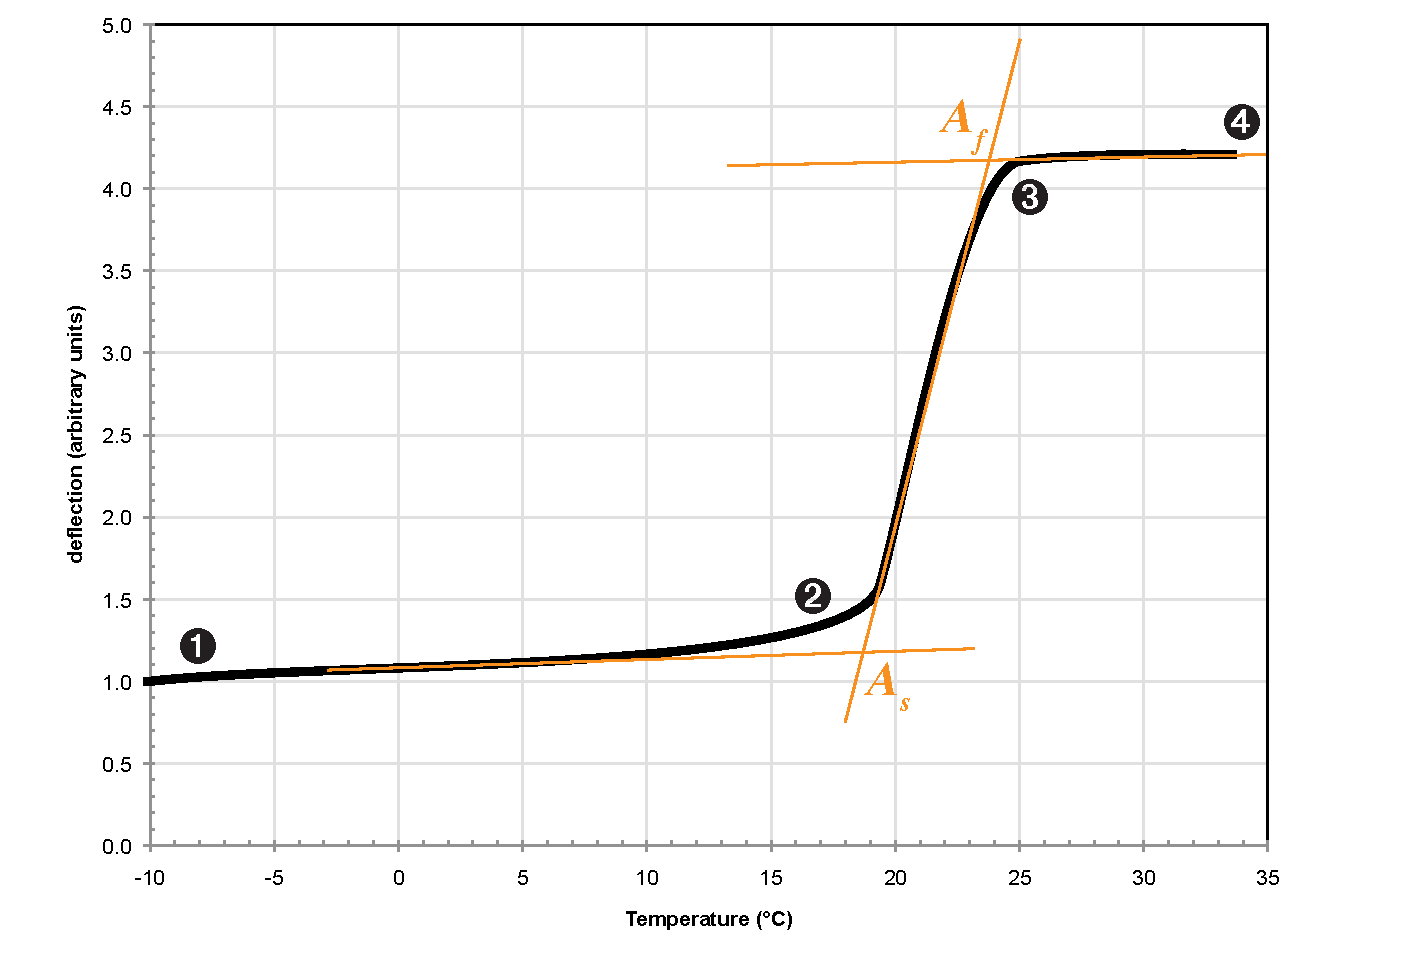
\includegraphics[width=0.9\textwidth]{./figs/af-test}
  \caption{Typical transition temperature measurement results, using a bend
  free recover technique}
  \label{fig:af-test}
\end{figure}

Figure \ref{fig:tensile} below illustrates
typical stress vs. strain response for superelastic Nitinol in a uniaxial
tensile test, for material having a transition temperature of approximately 25
degrees C. From position 1 to 2, the material is in its austenite phase. From
position 2 to 3, the material is undergoing a transition from austenite to
martnesite; this region is typically described as the \emph{upper plateau}. From
position 3 to 4, the material is fully martensitic; note that the slope in the
3-4 region is less steep than that in the 1-2 region, demonstrating the
relatively lower modulus of martensite compared with austenite. When material is
unloaded, it follows a different stress-strain path from position 4 to 5, then
transitions along the \emph{lower plateau} to position 6, before full recovering
to its original shape at position 1. 

% ^{\circ}\mathrm{C}.%

\begin{figure}[ht!]
  \centering 
  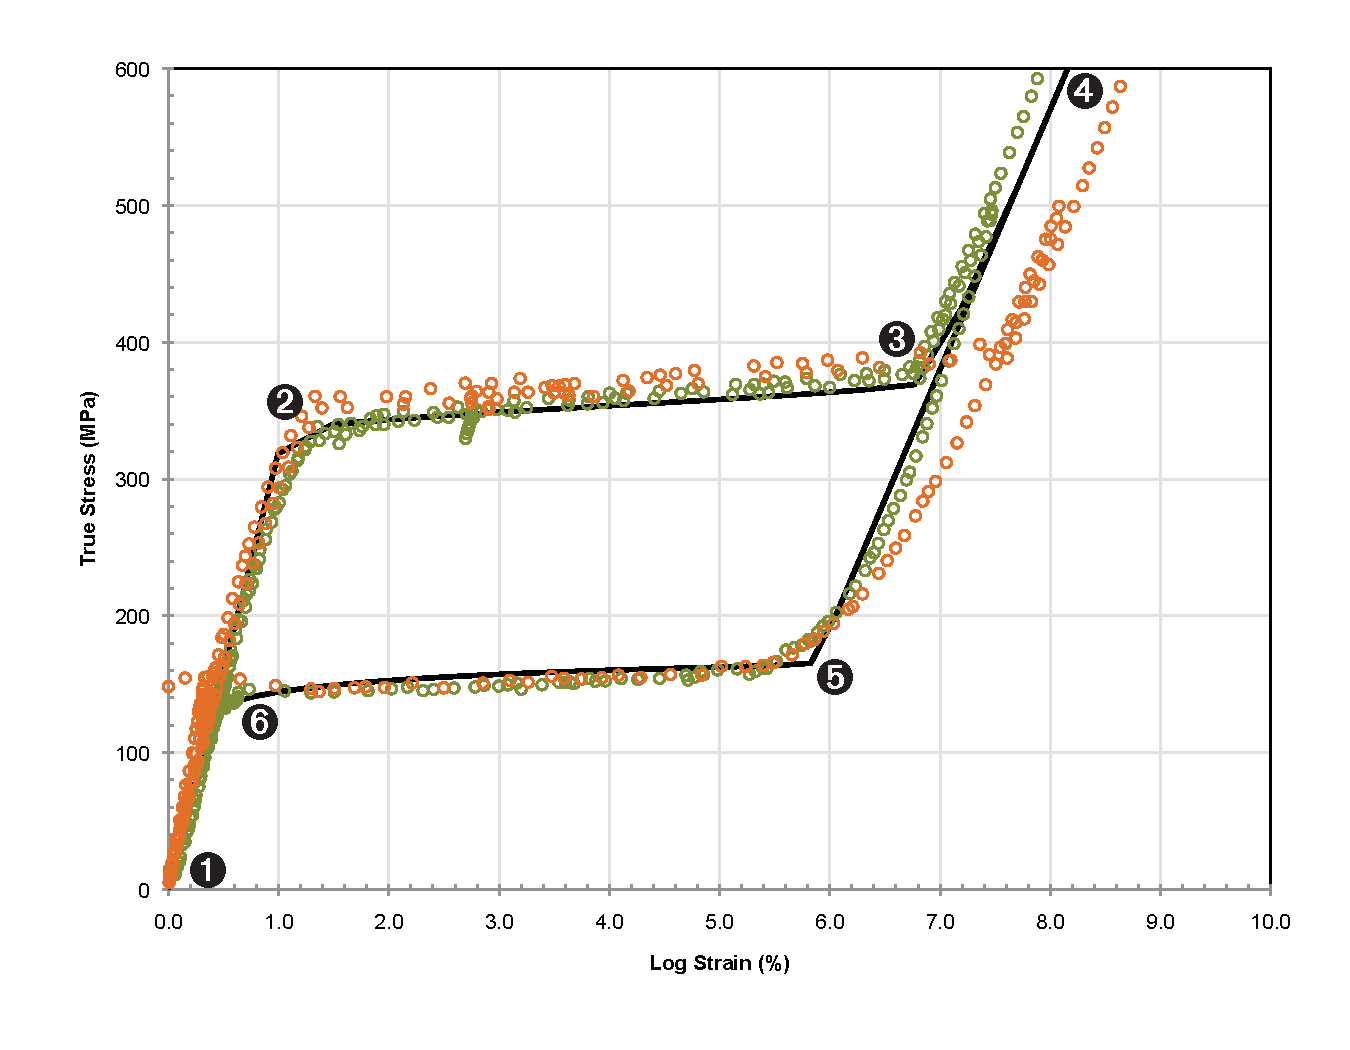
\includegraphics[width=0.9\textwidth]{./figs/tensile}
  \caption{Typical uniaxial tensile test data for superelastic
  Nitinol}
  \label{fig:tensile}
\end{figure}

The Stent Calculator formulations described later can theoretically apply to any
type of metallic stent, but are especially well suited to Nitinol designs. This
has nothing to do with the unusual shape memory or superelastic properties of
the material, but rather the unusually high strains that can be achieved in the
\emph{linear elastic} region of the austenite phase. The 
stress-strain curve between position 1 and 2 is substantialy linear for strains
of 1\% to 2\% in typical superelastic nitinol, which is an order of magnitude
higher than the comparable level of fully recovereable strain in conventional
engineering materials like stainless steel. Because of this, the stess vs.
strain relationship for nitinol stents is approximately constant for
relatively large, and often clinically relevant, range of deformations.

\section{Stent Anatomy}

Stents typically are comprised of an array of repeating structural elements
commonly described as \emph{struts}. These struts are generally oriented with
their long dimension aligned with the axis of the cylindrical form of the stent.
Struts are typically disposed around the circumference of a stent, and joined at
alternating ends to form a series of ``V'' or ``W'' shapes. The union of adjacent
struts is commonly described as a tip, elbow, or \emph{apex}. A series of struts
and apices that traverses one complete circumference is commonly described as a
ring or \emph{column}. Adjacent columns of struts are typically joined by
\emph{bridges} which connect some or all apices according to some regular
pattern.

\section{Transformations}

Stents experience some important transformations during fabrication and service.
Several of these are described in the following sections.

\subsection{Diameter Transformation} 

A stent must be able to transform from a small diameter during insertion and
delivery to a larger diameter at the implantation site, and in some cases repeat
this cycle one or more times. If the stent is designed at or near its intended
minimum diameter, the designer must craft features that can be fabricated at this
small diameter, and expand to the intended maximum diameter, while providing the
intended strength, scaffolding, flexibility and durability at a range of service
diameters. Alternatively, if a stent is designed and fabricated at or near its
maximum diameter, the designer must assure that the features can crimp, fold, or
otherwise pack efficiently allowing the structure to be constrained to the
intended minimum diameter. In both cases, it is very easy to design structures
that appear compelling in their fabricated state, but fail to transform to the
opposite end of the expansion range. To avoid this unsatisfying end, the stent
must be designed with both the \emph{crimped} and \emph{expanded} configuration
in mind.

\subsection{Material Removal} 

Another important transformation that occurs during manufacturing is
\emph{material removal}. Stents are commonly fabricated using a laser machining
process that leaves a heat affected zone (HAZ) of some thickness adjacent to cut
surfaces. Furthermore, the tubing from which stents are fabricated commonly have
draw lines or other undesired features on their inner or outer surfaces. For
these and other reasons, material is typically removed from the \emph{raw}, or
\emph{as-cut} component by some combination of mechanical or chemical processes.
Consequently, the stent must be designed to be fabricated according to one set of
feature dimensions, then processed to remove a specified amount of material from
each surface, such that the features achieve some desired \emph{finished}
dimensional targets. Here again, the stent must be designed with both the
\emph{raw} and \emph{finished} configuration in mind.

\subsection{Dimensionality and Coordinate Systems}

One additional transformation is simply an engineering abstraction, albeit an
important one. Stents are typically cylindrical structures that naturally exist
in a cylindrical coordinate system. However, they are typically designed in
planar form, using a cartesian coordinate system. Both are essential. The laser
cut pattern for a stent must be developed in a two dimensional planar form,
wherein the vertical height of the ``unwrapped'' stent is equivalent to the
circumference of the tube on which it will be cut. The motion controller that
reads the machine code will transform the vertical coordinates to \emph{theta}
coordinates, or rotational motions to fabricate the stent. While the two
dimensional planar representation is essential for fabrication, a three
dimensional cylindrical, or \emph{wrapped}, representation is helpful for
visualizing the actual component, and is essential for simulation and analysis.

\subsection{Simultaneous Configurations and Constraints}

Within a single instance of a single iteration of a single stent design, lie a
multitude of embodiments, all of which must be considered simultaneously to
achieve a successful design. The designer must consider:
\begin{itemize}
  \item Crimped and expanded diameter configurations
  \item Raw and finished feature dimensions
  \item Planar and cylindrical representations
  \item And more\ldots
\end{itemize}
Beyond these items, a design family may be comprised of a matrix of different
stent lengths and expansion diameters, and may have multiple design features
within a single stent. And it is likely that these features will be iterated many
times during the design and development process to achieve optimal performance,
reliability, and manufacturability. The combination of all of these simultaneous
configurations and constraints creates an important opportunity to apply the
tools of \emph{computer aided design}, or \emph{CAD}.

\section{Computer Aided Design of a nitinol Stent}

While Computer Aided Design, or CAD, has come to be associated with computerized
drafting or solid modeling, in a more general sense the term applies to any
computer based techniques that can be applied to the design or development
process. This manuscript considers three interrelated elements of computer aided
stent design. Each is driven by some essential design inputs, and provides some
prediction of relevant performance outputs.
\begin{enumerate}
  \item \textbf{Parametric Solid Modeling}: A three dimensional solid model is
  developed to programmatically create a stent design in any combination of
  crimped, expanded, raw, finished, planar or cylindrical forms. 
  \item \textbf{Stent Calculator}: A series of formulas is developed to predict
  the strength, strain, durability, and other performance features of a stent design
  on the basis of a finite set of input parameters. 
  \item \textbf{Finite Element Analysis}: The stent design is simulated using
  the techniques of finite element analysis to confirm the Stent Calculator results.
\end{enumerate}

Each of these are described in the following chapters. The order of the first two
is somewhat arbitrary, and does not imply dependency. Stent Calculator and the
Parametric Solid Model both require the same input data, and neither require the
results of the other. The tools of Stent Calculator are very easy to apply to
many ``what-if'' design scenarios very quickly, making it a very useful screening
tool. Consequently, it is best to explore many potential designs using Stent
Calculator before investing energy into any Parametric Solid Modeling. In any
event, Finite Element Analysis (FEA) is the most complex of the three, and is
typically used sparingly. In this manuscript, the Parametric Solid Modeling
chapter is presented first with the intention of providing a visual and geometric
basis for understanding the math and discussion in the later Stent Calculator
chapter.

\chapter{Parametric Solid Model}

It would be challenging to describe the design process for a stent without
referring to an actual stent design. Since virtually every every stent design in
existence is proprietary, a new generic design was created for this exercise. The
Open Source Stent (OSS) is designed for no particular purpose other than provide
a realistic example for utilizing the tools of computer aided stent design.

The Open Source Stent described here was designed with SolidWorks Professional
2010 (Dassault Syst\`emes SolidWorks Corporation, Concord, MA). SolidWorks is a
widely used commercial CAD software package that is commonly used in the medical
device industry. The source part file that is provided under the same terms as
this manuscript can be edited and manipulated with SolidWorks 2010 or higher, and
can be viewed using the eDrawings Viewer application available from
http://edrawingsviewer.com.

As noted in the previous chapter, the stent must be designed with a number of
simultaneous constraints in mind. This SolidWorks part is \emph{parameter}
driven, allowing the user to easily select the raw or finished state, crimped or
expanded state, and planar or wrapped configuration. The following sections
provide step by step details describing exactly how the stent geometry is built,
and how the model can be transformed between states. With the detail provided, a
moderately experienced user of Solidworks, or other solid CAD packages
(Pro/Engineer, Autodesk Inventor, or others) should be able to recreate the
design, and more importantly extend or customize the design to be suitable for
various applications. In the spirit of the Creative Commons, the community is
encouraged to create ``translated'' versions of this design, and share them with
the same licensing terms.

\section{Input Parameters and Equations}

\begin{table}[ht!] \caption{Global variables defined using SolidWorks equations} %
title name of the table \centering
\begin{tabular}{p{.6\textwidth} m{.4\textwidth}}
\\
\hline\hline 
Global Variable & Comment \\[0.5ex]
  \hline\hline
	\verb|"finishing"=1| & A logic flag to define whether the design is 
	in a raw/as-cut state (0) or finished state (1).\\
  \hline
	\verb|"expanded"=1| & A logic flag to define whether the design is in 
	a crimped state (0) or expanded state (1).\\
  \hline
	\verb|"N_col"=10| & Numer of columns of struts along the length of the 
	stent.\\
  \hline
	\verb|"N_struts"=42| & Number of struts around the circumference of the 
	stent.\\
  \hline
	\verb|"D_tube"=1.915| & Outer diameter of the tubing from which the 
	stent is cut.\\
 \hline
	\verb|"D_set"=8| & Expanded diameter of the stent. \\
  \hline
	\verb|"t_raw"=0.17| & Wall thickness of the tubing from which the 
	stent is cut. \\
  \hline
	\verb|"L_strut_inner"=1.2| & Length of the strut.\\
  \hline
	\verb|"w_apex_raw"=0.13| & Width of an apex in the raw state. \\
  \hline
	\verb|"X_bridge"=.15| & Axial gap between adjacent columns of struts \\
  \hline
	\verb|"Y_bridge"=0| & Circumferential offset for each bridge. \\
  \hline
	\verb|"w_bridge_raw"=0.125| & Width of a bridge in the raw state. \\
  \hline
	\verb|"N_bridges"=7| & Number of bridges around the circumference \\
  \hline
	\verb|"w_kerf"=0.025| & Minimum circumferential gap between struts in 
	the crimped state. \\
  \hline
	\verb|"m_width"=0.036| & Amount of material removal from feature widths.\\
  \hline
	\verb|"m_thickness"=0.059| & Amount of material removal from wall thickness.\\
  \hline\hline
\end{tabular} 
\label{tab:sw-vars} 
\end{table}


\begin{table}[ht!] 
\caption{Equations to define global variables linked to feature dimensions} % title name of the table
\centering 
\begin{tabular}{m{.6\textwidth} m{.4\textwidth}}
\\
\hline\hline 
Equation & Comment \\[0.5ex]
  \hline\hline
	\begin{verbatim}"D_model"=
	"D_tube"+"expanded"*("D_set"-"D_tube")\end{verbatim}
	& Diameter of the model, considering the state of the \verb+expanded+ logic flag.\\
  \hline
	\begin{verbatim}"Y_strut"=
	"D_model"*pi/"N_struts"
	\end{verbatim}
	& Circumferential distance occupied by a single strut at the analysis diameter.\\
  \hline
	\begin{verbatim}"w_strut"=
	(("D_tube"*pi)/"N_struts")
	-"w_kerf"-"m_width"*"finishing"
	\end{verbatim}
	& Width of a strut, considering the state of the \verb+finishing+ logic flag. \\
  \hline
	\begin{verbatim}"w_bridge"=
	"w_bridge_raw"-"m_width"*"finishing"
	\end{verbatim}
	& Width of a bridge, considering the state of the \verb+finishing+ logic flag. \\
  \hline
	\begin{verbatim}"w_apex"=
	"w_apex_raw"-"m_width"*"finishing"
	\end{verbatim}
	& Width of an apex, considering the state of the finishing logic flag. \\
  \hline
	\begin{verbatim}"t"=
	"t_raw"-"m_thickness"*"finishing"
	\end{verbatim}
	& Wall thickness, considering the state of the finishing logic flag. \\
  \hline
	\begin{verbatim}"inner_radius"=
	("w_kerf"+"m_width"*"finishing")/2
	\end{verbatim}
	& Inner radius of an apex\\
  \hline
	\begin{verbatim}"outer_radius"=
	"inner_radius"+"w_strut"
	\end{verbatim}
	& Outer radius of an apex\\
  \hline
	\begin{verbatim}"L_strut_rectangle"=
	"L_strut_inner"-"inner_radius"*2
	\end{verbatim}
	& Length of the perfectly rectangular section of a strut between apieces\\
  \hline
	\begin{verbatim}"D_inner"=
	"D_model"-("t"*2)
	\end{verbatim}& Inner diameter of the stent\\
\hline
%\hline
\end{tabular} 
\label{tab:sw-eqs} 
\end{table}

The variables and equations described by Tables \ref{tab:sw-vars} and
\ref{tab:sw-eqs} can all be defined before beginning any geometry creation. In
SolidWorks, the equations are entered by accessing \verb"Tools > Equations..."
from the menu. When defining dimensions in sketches and features, the driving
value can be linked to these global variables as shown in Figures
\ref{fig:sw-link1} and \ref{fig:sw-link2}. The completed global variables and
equations appear as shown in Figure \ref{fig:sw-equations}.

\begin{figure}[ht!]
  \centering 
  \includegraphics[width=0.8\textwidth]{./figs/sw/link_values1}
  \caption{Define dimension by selecting ``Link values\ldots''}
  \label{fig:sw-link1}
\end{figure}

\begin{figure}[ht!]
  \centering 
  \includegraphics[width=0.8\textwidth]{./figs/sw/link_values2}
  \caption{Select desired global variables to link to feature dimension.}
  \label{fig:sw-link2}
\end{figure}

\begin{figure}[ht!]
  \centering 
  \includegraphics[width=0.9\textwidth]{./figs/sw/00_equations}
  \caption{SolidWorks global variables and equations driving design features}
  \label{fig:sw-equations}
\end{figure}

\section{Master Strut Sketch}

The first sketch in the stent part is the \emph{Master Strut Sketch}. This sketch
is carefully constructed such that all of its feature dimensions are driven by
global variables, and it can reliably transform from the crimped to expanded
state, and raw to finished state, without ``breaking''. The sketch is fully
constrained without being overconstrained, which is a balance that can be
challenging to achieve with stent models in SolidWorks.

The sketch is created on the front plane, and the first geometry features placed
in the sketch form a rectangle comprised of \emph{construction lines}. The bottom
horizontal line is anchored at one end to the origin, and the top horizontal line
is placed at a distance of \verb"Y_strut" above the bottom line. These two lines
define the bounds of the strut in the vertical or circumferential direction, and
the spacing between them will vary depending upon the crimped or expanded
diameter of the stent. Vertical lines are then placed at the left and right,
forming a construction rectangle that will bound the strut at all times. Figure
\ref{fig:sketch-crimp} shows the master strut sketch in the crimped state, and
Figure \ref{fig:sketch-exp} shows the same master strut sketch in the expanded
state. Note that the horizontal length of the construction rectangle is not
defined, but rather it is dependent upon the defined length of the strut, and the
angle at which the strut is expanded. It should also be noted that the expanded
configuration assumes that the strut will be perfectly straight, while in reality
an expanded strut bend with a curvature that is too complex to represent in this
simple model. Consequently, the expanded configuration constructed in this CAD
model should be considered a visual approximation only.

\begin{figure}[ht!]
  \centering 
  \includegraphics[width=0.8\textwidth]{./figs/sw/01_sketch_crimp}
  \caption{Master strut sketch, with the model in the crimped state}
  \label{fig:sketch-crimp}
\end{figure}

\begin{figure}[ht!]
  \centering 
  \includegraphics[width=0.8\textwidth]{./figs/sw/02_sketch_exp}
  \caption{Master strut sketch, with the model in the expanded state}
  \label{fig:sketch-exp}
\end{figure}

\FloatBarrier

\section{Creating a Planar Unit Cell}

The first sketch is preserved as a ``master'', leaving it available for future
use if necessary. To achieve this, a new sketch is created for the first extrude
feature, and the ``convert entities'' function in the sketch module is used to
create new entities that are linked to those in the master sketch. With this
technique, no new dimensions are defined in the extrude feature, other than the
thickness of the extrusion itself (which is linked to the global variable
\verb"t"). The first strut is shown in Figure \ref{fig:extrude}. After creating
this first strut, it is mirrored to form a strut pair. In the next step, the
strut pair is copied twice. The number of ``copies'' to define in this step
depends on the pattern of bridge connections in the desired design. In this
42-strut case, there are seven bridges around the circumference, or one for every
three strut pairs; therefore, two copies are required for this design. The
mirrored, copied, and combined strut are shown in Figure \ref{fig:combine}.

Once the first set of struts has been created, the bridge features are added to
each end, as shown in Figure \ref{fig:bridge}. The combined structure now
represents half of the \emph{unit cell}, or smallest repeating geometry unit in
the stent. This structure is next copied in the axial direction, forming the
first elements of the second column of the design, as seen in Figure
\ref{fig:copy-struts}. The struts are now in an inconvenient arrangement, so a
split and move features are created to form the final combined planar unit cell
geometry as shown in Figure \ref{fig:realign-struts}

\begin{figure}[ht!]
  \centering 
  \includegraphics[width=0.8\textwidth]{./figs/sw/03_extrude}
  \caption{The first strut is extruded into solid form.}
  \label{fig:extrude}
\end{figure}

\begin{figure}[ht!]
  \centering 
  \includegraphics[width=0.8\textwidth]{./figs/sw/04_mirror_copy_combine}
  \caption{The strut is mirrored, copied, and combined.}
  \label{fig:combine}
\end{figure}

\begin{figure}[ht!]
  \centering 
  \includegraphics[width=0.8\textwidth]{./figs/sw/05_bridge_extrude}
  \caption{The bridge geometry is sketched and extruded.}
  \label{fig:bridge}
\end{figure}

\begin{figure}[ht!]
  \centering 
  \includegraphics[width=0.8\textwidth]{./figs/sw/06_copy_struts}
  \caption{The first partial column of struts is copied to form the second partial column.}
  \label{fig:copy-struts}
\end{figure}

\begin{figure}[ht!]
  \centering 
  \includegraphics[width=0.8\textwidth]{./figs/sw/07_realign_struts}
  \caption{The struts are realigned to form the final unit cell.}
  \label{fig:realign-struts}
\end{figure}

\FloatBarrier

\section{Creating a Full Planar Stent Model}

The unit cell geometry developed in the previous section is the repeating unit
that forms the basis for the full stent geometry. However, the ends of a stent
typically have some unique geometry features that require special treatment. At
very least, the bridges should not be present at the ends of the stent, so they
need to be removed. The approach, then, is to copy the unit cell in the axial
direction as many times as necessary, then modify the end features before copying
the full axial unit around the circumference. These steps are created in the same
SolidWorks part file, but using a new \emph{configuration}. With this approach,
the full model can build from the unit cell model, and when both are completed,
the user can easily switch between them.

Figure \ref{fig:axial-copy} shows the first axial copying step,\footnote{Using a
\emph{Linear Pattern} feature may be more obvious and intuitive, but this feature
does not allow the offset distance to be derived directly from existing geometry.
With the \emph{Body Move/Copy} feature, corresponding points at the right and
left bridges are used to define the translation for each copy. Now, as the
geometry is modified, these points move automatically, and the copy feature
always uses the correct translation.} in this case creating four copies of the
first pair of columns, for a total of ten columns in the finished design. To
correct the geometry at each end, the strut pairs are \emph{split} in such as way
that the apex with the bridge can be deleted with a \emph{Delete Body}, and the
apex without the bridge can be copied in its place with a \emph{Body Move/Copy}
feature. These steps are shown in Figures \ref{fig:split} and
\ref{fig:copy-apex}. Finally, the geometry is patterned around the circumference
using copy and combine features, with the final result shown in Figure
\ref{fig:full-planar}.

\begin{figure}[ht!]
  \centering 
  \includegraphics[width=0.8\textwidth]{./figs/sw/08_axial_copy}
  \caption{Master strut sketch, with the model in the crimped state.}
  \label{fig:axial-copy}
\end{figure}

\begin{figure}[ht!]
  \centering 
  \includegraphics[width=0.8\textwidth]{./figs/sw/09_split}
  \caption{Defining the split feature. Prior to this step, a reference plane was created 
  by selecting the midpoints of the struts shown. Now, the split feature is always positioned 
  at the correct location on the strut.}
  \label{fig:split}
\end{figure}

\begin{figure}[ht!]
  \centering 
  \includegraphics[width=0.8\textwidth]{./figs/sw/10_copy_apex}
  \caption{After deleting the apex with the unwanted bridge, 
  the clean apex is copied into place.}
  \label{fig:copy-apex}
\end{figure}

\begin{figure}[ht!]
  \centering 
  \includegraphics[width=0.8\textwidth]{./figs/sw/11_full_planar}
  \caption{The full planar stent geometry, ready to 
  create a two dimensional CAD file for laser coding.}
  \label{fig:full-planar}
\end{figure}

\FloatBarrier

\section{Creating a Wrapped Unit Cell Model}

As described in the previous section, the wrapped unit cell model is created as a
new configuration that builds upon the planar unit cell shown above in Figure
\ref{fig:realign-struts}. The first step in building this configuration is to
actually delete the planar unit cell using the \emph{Delete Body} feature, as
seen in Figure \ref{fig:delete-unitcell}. Next, in Figure \ref{fig:cylinder}, a
cylinder is created, onto which the unit cell geometry will be projected and
embossed. A \emph{Wrap} feature is created, along with a new sketch on the front
plane. While in this sketch, the deleted final planar unit cell geometry is
selected from the model tree. One face is selected, the \emph{Convert Entities}
function in the sketch module traces the unit cell, and creates new cloned
geometry for the wrap feature that is linked back to the original planar unit
cell, shown in Figure \ref{fig:clone}. When the wrap feature is completed, the
unit cell geometry becomes embossed on the inner surface of the cylinder, as
shown in Figure \ref{fig:wrap}. Next, in Figure \ref{fig:cut-cylinder}, the
cylinder is cut away, leaving behind the finished wrapped unit cell, as shown in
Figure \ref{fig:wrap-unitcell}.

\begin{figure}[ht!]
  \centering 
  \includegraphics[width=0.8\textwidth]{./figs/sw/12_delete_unitcell}
  \caption{The planar unit cell is deleted from the model, but can still be used 
  later to define the wrapping geometry.}
  \label{fig:delete-unitcell}
\end{figure}

\begin{figure}[ht!]
  \centering 
  \includegraphics[width=0.8\textwidth]{./figs/sw/13_cylinder}
  \caption{A cylinder with its inner diameter equal to the desired outer 
  diameter of the wrapped stent. The thickness of this cylinder is arbitrary.}
  \label{fig:cylinder}
\end{figure}

\begin{figure}[ht!]
  \centering 
  \includegraphics[width=0.8\textwidth]{./figs/sw/14_clone_unitcell}
  \caption{A clone of the unit cell is created by linking features in a new
  sketch back to the planar unit cell created above.}
  \label{fig:clone}
\end{figure}

\begin{figure}[ht!]
  \centering 
  \includegraphics[width=0.8\textwidth]{./figs/sw/15_wrap}
  \caption{The unit cell is projected onto the inner surface of the cylinder and 
  embossed to create a wrapped unit cell.}
  \label{fig:wrap}
\end{figure}

\begin{figure}[ht!]
  \centering 
  \includegraphics[width=0.8\textwidth]{./figs/sw/16_extrude}
  \caption{The cylinder is stripped away from the unit cell using a cut feature.}
  \label{fig:cut-cylinder}
\end{figure}

\begin{figure}[ht!]
  \centering 
  \includegraphics[width=0.8\textwidth]{./figs/sw/17_wrapped_unitcell}
  \caption{The final wrapped unit cell.}
  \label{fig:wrap-unitcell}
\end{figure}

\FloatBarrier

\section{Creating a Full Wrapped Model}

The fourth and final configuration to create is a full wrapped stent model. The
process for creating this model is similar to that used to extend the planar unit
cell model to a full planar model above. First, in Figure
\ref{fig:wrapped-axial-copy}, the wrapped unit cell is patterned in the axial
direction using \emph{Body Move/Copy} as before. Next, in Figure
\ref{fig:wrapped-delete-apex}, the struts are split, and the unwanted apex is
deleted. For the next step, the new apex can not be simply translated to the
empty place as before; rather, it must be translated \emph{and rotated} to align
properly. To accomplish this, the apex is first copied to an area away from the
stent, as shown in Figure \ref{fig:wrapped-copy-apex}. This detached apex is next
moved into place using \emph{mating} functionality of \emph{Body
Move/Copy}\footnote{Unfortunately, SolidWorks does not allow mating alignments
when \emph{copying} bodies \--- this only works when \emph{moving bodies}. It is
for this reason that the intermediate step of creating a detached apex is
required.}. As shown in Figure \ref{fig:wrapped-mate-apex} two pairs of
coincident points are selected on the detached apex and the stent itself. This
provides adequate constraints to position the new apex properly. This is repeated
on both ends of the stent. In Figure \ref{fig:wrapped-axis}, an axis is created
at the intersection of the top and front planes to define the central axis of the
stent. Finally, in Figure \ref{fig:circ-pattern}, the \emph{Circular Pattern}
feature is used to complete the wrapped stent geometry. After a final
\emph{combine} feature, the full wrapped stent geometry can be seen in Figure
\ref{fig:full-wrap}.

\begin{figure}[ht!]
  \centering 
  \includegraphics[width=0.8\textwidth]{./figs/sw/18_wrapped_axial_copy}
  \caption{The wrapped unit cell is copied in the axial direction.}
  \label{fig:wrapped-axial-copy}
\end{figure}

\begin{figure}[ht!]
  \centering 
  \includegraphics[width=0.8\textwidth]{./figs/sw/19_delete_apex}
  \caption{After splitting the strtus, the unwanted apex is deleted.}
  \label{fig:wrapped-delete-apex}
\end{figure}

\begin{figure}[ht!]
  \centering 
  \includegraphics[width=0.8\textwidth]{./figs/sw/20_copy_apex}
  \caption{The new apex is copied away from the stent temporarily.}
  \label{fig:wrapped-copy-apex}
\end{figure}

\begin{figure}[ht!]
  \centering 
  \includegraphics[width=0.8\textwidth]{./figs/sw/21_mate_apex}
  \caption{The detached apex is moved into place using to coincident point pairs.}
  \label{fig:wrapped-mate-apex}
\end{figure}

\begin{figure}[ht!]
  \centering 
  \includegraphics[width=0.8\textwidth]{./figs/sw/22_axis}
  \caption{An axis is placed at the center of the stent.}
  \label{fig:wrapped-axis}
\end{figure}

\begin{figure}[ht!]
  \centering 
  \includegraphics[width=0.8\textwidth]{./figs/sw/23_circ_pattern}
  \caption{A circular pattern feature completes the circumferential patterning.}
  \label{fig:circ-pattern}
\end{figure}

\begin{figure}[ht!]
  \centering 
  \includegraphics[width=0.8\textwidth]{./figs/sw/24_final_full_wrap}
  \caption{The final fully wrapped stent.}
  \label{fig:full-wrap}
\end{figure}

\FloatBarrier

\section{Transforming the State of the Model}

The completed solid part can now be easily transformed into alternate
configurations. To change from the raw to the finished state, change the
\verb"finishing" global variable from \verb"0" to \verb"1", as shown in Figure
\ref{fig:finishing}. After making the change, the user must manually trigger a
rebuild of the model by clicking the appropriate icon, or pressing \verb"Ctrl+B".
The transformed finished part is shown in Figure \ref{fig:finished}. To change
from the crimped to expanded state, change the \verb"expanded" global variable
from \verb"0" to \verb"1", as shown in Figure \ref{fig:expanding}. After
rebuilding the model, the result is shown in Figure \ref{fig:expanded}.

The wrapped and planar state, as well as the unit cell and full states for each,
are controlled by SolidWorks \emph{Configurations}.\footnote{Ideally, the
crimped or expanded state, and raw or finished state would also be controlled by
\emph{Configurations} Unfortunately, this is not possible because of a
limitation that prevents global variables from being controlled in a
configuration design table. Reference SolidWorks Knowledge Base issue S-04428:
``Can a design table establish global variables which are used in SolidWorks
equations?''}. Figure \ref{fig:config-wrapunit} shows the configuration selection
for the wrapped unit cell case, and Figure \ref{fig:config-planarunit} shows the
configuration selection for the planar unit cell case. Figure
\ref{fig:unit-cell-configs} depicts four possible unit cell configurations in the
crimped state. The bottom right case, a wrapped unit cell with finished
dimensions, is one that might be used for finite element analysis simulation.
Figure \ref{fig:planar-full-raw-crimp} is a planar full stent, in the crimped
configuration, with raw dimensions \--- this is a configuration that might be
used to generate a laser cutting program.  Finally, Figure
\ref{fig:wrap-full-fin-exp} depicts the full stent in its finished state \---
this configuration might be used to support a finished specification for the
component.

\begin{figure}[ht!]
  \centering 
  \includegraphics[width=0.8\textwidth]{./figs/sw/25_finishing}
  \caption{Change from the raw to finished state by editing 
  the ``finishing'' global variable.}
  \label{fig:finishing}
\end{figure}

\begin{figure}[ht!]
  \centering 
  \includegraphics[width=0.8\textwidth]{./figs/sw/26_finished}
  \caption{Transformation to the finished state.}
  \label{fig:finished}
\end{figure}

\begin{figure}[ht!]
  \centering 
  \includegraphics[width=0.8\textwidth]{./figs/sw/27_expanding}
  \caption{Change from the crimped to expanded state by editing the
  ``expanded'' global variable.}
  \label{fig:expanding}
\end{figure}

\begin{figure}[ht!]
  \centering 
  \includegraphics[width=0.8\textwidth]{./figs/sw/28_expanded}
  \caption{Transformation to the expanded state.}
  \label{fig:expanded}
\end{figure}

\begin{figure}[ht!]
  \centering 
  \includegraphics[width=0.8\textwidth]{./figs/sw/29_config_wrapunit}
  \caption{Change to the wrapped unit cell state using the SolidWorks 
  configuration manager.}
  \label{fig:config-wrapunit}
\end{figure}

\begin{figure}[ht!]
  \centering 
  \includegraphics[width=0.8\textwidth]{./figs/sw/30_config_planarunit}
  \caption{Change to the planar unit cell state using the SolidWorks 
  configuration manager.}
  \label{fig:config-planarunit}
\end{figure}

\begin{figure}[ht!]
  \centering 
  \includegraphics[width=0.95\textwidth]{./figs/sw/unit-cell-configs}
  \caption{Crimped unit cell configurations. Top: Planar.  
  Bottom: Cylindrical. Left: Raw. Right: Finished.}
  \label{fig:unit-cell-configs}
\end{figure}

\begin{figure}[ht!]
  \centering 
  \includegraphics[width=0.95\textwidth]{./figs/sw/planar_full_raw_crimp}
  \caption{Planar full stent, in the raw state. This geometry is 
  suitable for laser cutting.}
  \label{fig:planar-full-raw-crimp}
\end{figure}

\begin{figure}[ht!]
  \centering 
  \includegraphics[width=0.95\textwidth]{./figs/sw/wrap_full_fin_exp}
  \caption{Cylindrical full stent, in the finished state. This geometry is 
  suitable for supporting a final component specification.}
  \label{fig:wrap-full-fin-exp}
\end{figure}

\FloatBarrier


\chapter{Stent Calculator Formulas}

This chapter details the variables and formulas used in the Stent Calculator
application. Each section focuses on a specific aspect of design or performance,
and generally the results from each section are used for further calculations in
later sections. Throughout this text, example values are provided based on the
Open Source Stent design described in the previous section. Where applicable, the
example values are provided with corresponding SI units of measure.

\section{Stent Design Inputs}
The variables below define the key aspects of stent geometry. These inputs are
typically drawn from an engineering drawing or related specification.

$N_{col}$ is the number of columns of struts along the length of the stent.

\begin{align} 
	N_{col}  = 10
\end{align}	

$N_{struts}$ is the number of columns of struts around the circumference 
of the stent.

\begin{align}
\begin{split}
	N_{struts}  = 42
\end{split}
\end{align}	

$D_{tube}$ is the outer diameter of the tube from which the stent is 
fabricated, in millimeters.

\begin{align}
\begin{split}
	D_{tube}  = 1.915 \text{ mm}
\end{split}
\end{align}	

$t_{raw}$ is the wall thickness of the tube from which the stent is fabricated,
in millimeters.

\begin{align}
\begin{split}
	t_{raw}  = 0.17 \text{ mm}
\end{split}
\end{align}	

$L_{strut\_inner}$ is the length of a strut, as measured between the quadrants of
the inner arcs of opposite apices, in millimeters.

\begin{align}
\begin{split}
	L_{strut\_inner}  = 1.200 \text{ mm}
\end{split}
\end{align}	

$w_{apex\_raw}$ is the width of an apex in the raw, or as-cut, state. This width
may be equal to the strut width, but it does not necessarily need to be. It is
often designed to be some multiple of a strut width (\emph{i.e.} 1.0x, 1.1x,
1.2x, etc.).

\begin{align}
\begin{split}
	w_{apex\_raw}  = 0.130 \text{ mm}
\end{split}
\end{align}	

$X_{bridge}$ is the axial gap between adjacent columns of struts, as measured by
the axial distance between the closest points on the outer arc of adjacent
apices.

\begin{align}
\begin{split}
	X_{bridge}  = 0.125 \text{ mm}
\end{split}
\end{align}	

$Y_{bridge}$ is the circumferential distance traversed by a single bridge, or the
offset in the circumferential direction between like points of corresponding
adjacent apices.

\begin{align}
\begin{split}
	Y_{bridge}  = 0.000 \text{ mm}
\end{split}
\end{align}	

$w_{bridge\_raw}$ is the width of a bridge element in the raw, or as-cut, state.

\begin{align}
\begin{split}
	w_{bridge\_raw} = 0.125 \text{ mm}
\end{split}
\end{align}

$N_{bridges}$ is the number of bridges around the circumference of the stent.
Typically, this value must be a factor of $\dfrac{N_{struts}}{2}$. In the case of
this example, with 42 struts, $N_{bridges}$=21 would imply that every internal
apex is connected to an adjacent apex. $N_{bridges}$=7 would imply that every
third internal apex is connected to a corresponding adjacent apex. The only other
option, $N_{bridges}$=3 suggests that every seventh internal apex is connected.

\begin{align}
\begin{split}
	N_{bridges} = 7
\end{split}
\end{align}

\begin{figure}[hbtp]
  \centering 
  \includegraphics[width=0.8\textwidth]{./figs/unit-cell-ascut.pdf}
  \caption{Unit cell stent geometry in the raw, or as-cut, state}
  \label{fig:unit-cell-ascut}
\end{figure}

\begin{figure}[hbtp]
  \centering 
  \includegraphics[width=0.8\textwidth]{./figs/unit-cell-expanded}
  \caption{Unit cell stent geometry in the expanded and finished state}
  \label{fig:unit-cell-expanded}
\end{figure}

\section{Stent Process Inputs}
The variables below relate to various assumptions regarding the manufacturing
processes used to fabricate the stent.

$w_{kerf}$ is the effective kerf width between struts when fabricated (or in the
crimped state). In the typical case of laser micromachining of stent from tubing,
this is the effective width of the laser beam.

\begin{align}
\begin{split}
	w_{kerf}  = 0.025 \text{ mm}
\end{split}
\end{align}	

$m_{width}$ is the total amount of material removal from feature widths during
finishing operations, i.e. after laser cutting is complete. Typically, the raw
feature widths are planned to be larger than finished feature widths to allow for
effective removal of the \emph{heat affected zone}, or HAZ, of material that may
be embrittled by the cutting operation. $m_{width}$ is selected to allow for HAZ
removal, as well as provide for sufficient surface smoothing and edge rounding as
required by the design.

\begin{align}
\begin{split}
	m_{width}  = 0.036 \text{ mm}
\end{split}
\end{align}	

$m_{thickness}$ is the total amount of material removal from the wall thickness
during finishing operations, i.e. after laser cutting is complete. This is
commonly greater than $m_{width}$ because is it often desirable to remove
additional material from the inner surface of the stent to eliminate tubing draw
lines or other unwanted surface features from the inner and/or outer surfaces of
the stent.

\begin{align}
\begin{split}
	m_{thickness}  = 0.059 \text{ mm}
\end{split}
\end{align}	

$A_f$ is the austenite finish temperature of the finished component. This is the
temperature at which the transformation from martensite to austenite is complete,
as measure by bend free recovery techniques.
\begin{align}
\begin{split}
	A_f  = 27  ^{\circ}\mathrm{C}
\end{split}
\end{align}	

\section{Material Property Inputs}

The Stent Calculator application is particularly well suited to analyze nitinol
designs because of the unique �linear elastic� behavior of the material with
strains of 1-2\%. In this regime, the material is dominated by the properties of
the austenite phase. The elastic modulus of this material in this phase varies
with the transformation temperature. With $A_f$ temperatures progressively lower
than body temperature, the stiffness of the material at body temperature
increases (See Figure  \ref{fig:modulus-temperature}). Understanding this
relationship, Stent Calculator can adjust the elastic modulus of the material as
a function of specified $A_f$ temperatures using the curves fit to data as shown
in Figure \ref{fig:modulus-temperature}.

\begin{figure}[hbtp]
  \centering
  \includegraphics[width=0.8\textwidth]{./figs/e_vs_Af.pdf} 
  \caption{Relationship between initial (austenite) modulus and $A_f$
  temperature for superelastic nitinol at an environmental temperature of 
  $37^{\circ}\mathrm{C}$. The points shown were obtained experimentally from
  nitinol tubing heat treated to achieve desired $A_f$ temperatures. The green 
  and orange curves were developed manually to fit the
  data, and reasonably reflect the expected performance of the material. The
  green curve applies for $A_f$ temperatures less than $19^{\circ}\mathrm{C}$,
  and the orange curve applies for $A_f$ temperatures greater than
  $19^{\circ}\mathrm{C}$.}
  \label{fig:modulus-temperature}
\end{figure}

$E_{Af,low}$ is the elastic modulus of the austenite phase having an $A_f$
temperature of $Af_{low}$.
\begin{align}
\begin{split}
	E_{Af,low}  = 94,000 \text{ MPa}
\end{split}
\end{align}	

$Af_{low}$ is the first $A_f$ temperature at which the austenite elastic modulus
is defined.
\begin{align}
\begin{split}
	Af_{low}  = -5  ^{\circ}\mathrm{C}
\end{split}
\end{align}

$E_{Af,high}$ is the elastic modulus of the austenite phase having an $A_f$
temperature of $Af_{high}$.
\begin{align}
\begin{split}
	E_{Af,high}  = 34,000 \text{ MPa}
\end{split}
\end{align}	

$Af_{high}$ is the second $A_f$ temperature at which the austenite elastic
modulus is defined.
\begin{align}
\begin{split}
	Af_{high}  = 37  ^{\circ}\mathrm{C}\\
\end{split}
\end{align}	

$Af_{inflection}$ is the temperature at which the $Af$ vs $E$ relationship
transitions from the low temperature curve to the high temperature curve, as
shown in Figure \ref{fig:modulus-temperature}.
\begin{align}
\begin{split}
	Af_{inflection}  = 19  ^{\circ}\mathrm{C}\\
\end{split}
\end{align}	

The calculated value of $E$, the austenite elastic modulus for a material
having the specified $A_f$, depends on the $A_f$ temperature. For $A_f$ less
than $Af_{low}$:

\begin{align}
	E_{case1} ={}& E_{Af,low}
\end{align}	

%
% EDIT - AL Comment: Change this figure to have solid / dashed lines
%

For $A_f$ between $Af_{low}$ and $Af_{inflection}$, the green curve of Figure
\ref{fig:modulus-temperature} applies:

\begin{align}
\begin{split}
	E_{case2} ={}& E_{Af,low} - 1.9 \cdot \left( A_f - Af_{low} \right)^3
\end{split}
\end{align}	

For $A_f$ between $Af_{inflection}$ and $Af_{high}$, the orange curve of Figure
\ref{fig:modulus-temperature} applies:

\begin{align}
\begin{split}
	E_{case3} ={}& E_{Af,high} + 5.9 \cdot \left( Af_{high} - A_f \right)^3
\end{split}
\end{align}	

For $A_f$ equal to or above $Af_{high}$:

\begin{align}
\begin{split}
	E_{case4} ={}& E_{Af,high}
\end{split}
\end{align}	

In this example, with $A_f = 27$, $E_{case3}$ applies.

\begin{align}
\begin{split}
	E ={}& E_{case3} \text{ for } A_f = 27  ^{\circ}\mathrm{C}\\
	E ={}& 34059 \text{ MPa}
\end{split}
\end{align}

$\rho$ is the mass density of nitinol, used later to estimate the mass of the
stent on the basis of its estimated volume.

\begin{align}
\begin{split}
	\rho ={}& 6.7 g/cm^3\\
	\rho ={}& 6.7 mg/mm^3
\end{split}
\end{align}	

$\epsilon_{fsl}$ is the fatigue strain limit of the material. For mean strains
less than 4\%, Pelton \emph{et. al.} report a strain amplitude fatiuge strain
limit of 0.4\% for nitinol test samples fabricated and processed using techniques
representative of those used for stents.\cite{Pelton:2008bd}
\begin{align}
\begin{split}\label{eq:endurance-limit}
	\epsilon_{fsl} = 0.4\%
\end{split}
\end{align}

\section{Service Parameters}
This section defines the diameter to which the stent is expanded, and the
diameter of the vessel into which the stent is placed. The �Analysis Diameter� is
also defined here, typically equal to the vessel diameter. Various properties of
the stent, including strength and strain, are calculated at this diameter.

This section also defines the mechanical properties of the vessel into which the
stent is placed. Commonly, the compliance of a vessel is reported in terms of a
percentage change in diameter related to a specific applied pressure range. This
compliance is typically defined based on arterial, venous, or other data derived
experimentally or drawn from literature. The systolic and diastolic pressures
considered in the fatigue analysis are also defined in this section.

$D_{set}$ is the expanded, or thermal shape set, diameter of the stent. This is
the maximum diameter to which the stent is expanded for any given usage case.

\begin{align}
\begin{split}
	D_{set} = 8.0 \text{ mm}
\end{split}
\end{align}

$D_{ves}$ is the diameter of the vessel into which the stent is placed. This is
typically smaller than $D_{set}$, the fully expanded diameter of the vessel. In
this example, the stent is \emph{oversized} by 1.5mm.

\begin{align}
\begin{split}
	D_{ves} = 6.5 \text{ mm}
\end{split}
\end{align}

$D$ is the diameter at which strains are calculated.

\begin{align}
\begin{split}
	D = D_{ves} = 6.5 \text{ mm}
\end{split}
\end{align}

$C_{percent}$ is part of the definition for vessel compliance. This is the
percent change in effective diameter for a defined change in pressure,
$C_{pressure}$. In the literature, this is often reported as $\Delta D / D$. The
compliance in this example is arbitrary, but similar to values commonly used in
the arterial system.

\begin{align}
\begin{split} \label{eq:c-percent}
	C_{percent} = 6\%
\end{split}
\end{align}

$C_{pressure}$ is part of the definition for vessel compliance. This is the
change in pressure\footnote{This is an arbitrary value, not necessarily related
to a physiologic pressure. Rather, it is simply the pressure half of the
definition for compliance, as reported in literature or by experiment} that is
related to a $\Delta D / D = C_{percent}$.

\begin{align}
\begin{split} \label{eq:c-pressure}
	C_{pressure} = 100 \text{ mmHg}
\end{split}
\end{align}

$P_{systolic}$ is the systolic pressure experienced at the site of stent
implantation.

\begin{align}
\begin{split}
	P_{systolic} = 150 \text{ mmHg}
\end{split}
\end{align}


$P_{diastolic}$ is the diastolic pressure experienced at the site of stent
implantation.

\begin{align}
\begin{split}
	P_{diastolic} = 50 \text{ mmHg}
\end{split}
\end{align}

%
% AL EDIT: Common formulaiton = 1/3 Psystole + 2/3 Pdiastole
%

$P_{mean}$ is the mean pressure experienced at the site of stent
implantation, assuming a simple sinusoidal pressure wave.

\begin{align}
\begin{split}
	P_{mean} = \dfrac{P_{systolic}+P_{disatolic}}{2}\\
	P_{mean} = 100 \text{ mmHg}
\end{split}
\end{align}


\section{Stent Dimension Calculations}

This section explains the calculations of a number of derived stent
characteristics and dimensions.

$N_{cells}$ is the number of ``crowns,'' ``tips,'' or ``\emph{cells}'' around
the circumference of the stent. This is equal to half the number of struts around the
circumference.

\begin{align}
\begin{split}
	N_{cells} ={}&  \frac{N_{struts}}{2}\\
	N_{cells} ={}& 21
\end{split}
\end{align}

$D_{crimp}$ is the fully constrained outer diameter of the stent within its
delivery sheath.

\begin{align}
\begin{split}
	D_{crimp} ={}& D_{tube}\\
	D_{crimp} ={}& 1.915 \text{ mm}
\end{split}
\end{align}

$L_{strut}$ is the effective length of the strut, as measured between the
centerlines of opposite apices. This measurement is not easily measured or
defined, so it is derived here based on the inner strut length and the width of
the apices in the raw state.

\begin{align}
\begin{split}
	L_{strut} ={}& L_{strut\_inner}+2\cdot \frac{w_{apex\_raw}}{2}\\
	L_{strut}={}& 1.330 \text{ mm}
\end{split}
\end{align}

$w_{strut_{raw}}$ is the width of each strut in the as-cut, or raw, state. This
value is derived based on the tubing diameter, number of struts around the
circumference, and the kerf width.

\begin{align}
\begin{split}
	w_{strut\_raw} ={}& \frac{D_{tube}\cdot \pi}{N_{struts}}-w_{kerf}\\
	w_{strut\_raw} ={}& 0.118 \text{ mm}
\end{split}
\end{align}

$w_{strut}$ is the width of each strut in the finished state. 

\begin{align}
\begin{split}
	w_{strut} ={}& w_{strut\_raw}-m_{width}\\
	w_{strut} ={}& 0.082 \text{ mm}
\end{split}
\end{align}

$w_{bridge}$ is the width of each bridge in the finished state. 

\begin{align}
\begin{split}
	w_{bridge} ={}& w_{bridge\_raw}-m_{width}\\
	w_{bridge} ={}& 0.089 \text{ mm}
\end{split}
\end{align}


$w_{apex}$ is the width of each apex in the finished state. 

\begin{align}
\begin{split}
	w_{apex} ={}& w_{apex\_raw}-m_{width}\\
	w_{apex} ={}& 0.094 \text{ mm}
\end{split}
\end{align}

$t$ is the wall thickness of the stent in the finished state. 

\begin{align}
\begin{split}
	t ={}& t_{raw}-m_{thickness}\\
	t ={}& 0.111 \text{ mm}
\end{split}
\end{align}

\section{Strut Angle and Deflection Calculations}
This section calculates a variety of derived strut angle and deflection
calculations. Angles and deflections are calculated here for the vessel 
diameter, and for a diameter 1mm less than the fully expanded diameter.

$\theta_{set}$ is the angle a single strut is deflected between the 
crimped state and the fully expanded (thermal shape set) state.

\begin{align}
\begin{split}
	\theta_{set} ={}& \left( \dfrac{180}{\pi } \right)\sin 
		\left[ \frac{\dfrac{D_{set}\cdot \pi -D_{crimp}\cdot\pi}
		{N_{struts}}}{L_{strut}} \right]\\
	\theta_{set} ={}& 20.0 \text{ degrees}
\end{split}
\end{align}

$\theta_{d}$ is the angle a single strut is deflected between the crimped 
state and the analysis diameter.

\begin{align}
\begin{split} \label{eq:theta-d}
	\theta_{d} ={}& \left( \frac{180}{\pi } \right)\sin 
		\left[ \dfrac{\dfrac{D\cdot \pi -D_{crimp}\cdot\pi}
		{N_{struts}}}{L_{strut}} \right]\\
	\theta_{d} ={}& 14.9 \text{ degrees}
\end{split}
\end{align}

$\Delta\theta_{d}$ is the change in angle of a single strut between the 
fully expanded diameter and the analysis diameter.

\begin{align}
\begin{split}\label{eq:delta-theta-d}
	\Delta\theta_{d} ={}& \theta_{set} - \theta_d\\
	\Delta\theta_{d} ={}& 5.1 \text{ degrees}
\end{split}
\end{align}

$2\theta$ is the maximum included angle, or the angle between a pair of
circumferentially adjacent struts in the expanded state.

\begin{align}
\begin{split}
	2\theta={}& 2\cdot\theta_{set}\\
	2\theta={}& 40.0 \text{ degrees}
\end{split}
\end{align}

$\delta_d$ is the deflection of a single strut between the expanded state
and the analysis diameter.

\begin{align}
\begin{split} \label{eq:delta-d}
	\delta_d ={}& 2\cdot L_{strut}\cdot \sin\left(\frac{\Delta\theta_d}{2}\right)\\
	\delta_d ={}& 0.118 \text{ mm}
\end{split}
\end{align}

$\theta_{1mm}$ is the deflection of a single strut between the expanded 
state and one millimeter less than the expanded diameter.

\begin{align}
\begin{split}
	\theta_{1mm} ={}&  \left(\dfrac{180}{\pi}\right) \sin 
		\left[ \displaystyle \dfrac{\dfrac{\left(  D_{set}-1 \right) 
		\cdot \pi -D_{crimp}\cdot\pi}{N_{struts}}}{L_{strut}} \right]\\
	\theta_{1mm} ={}& 16.6 \text{ deg}
\end{split}
\end{align}

$\Delta\theta_{1mm}$ is the change in angle of a single strut between 
the fully expanded diameter and one millimeter less than the expanded diameter.

\begin{align}
\begin{split}
	\Delta\theta_{1mm} ={}& \theta_{set} - \theta_{1mm}\\
	\Delta\theta_{1mm} ={}& 3.4 \text{ degrees}
\end{split}
\end{align}

$\delta_{1mm}$ is the deflection of a single strut between the expanded state and
one millimeter less than the expanded diameter.

\begin{align}
\begin{split}
	\delta_{1mm} ={}& 2\cdot L_{strut}\cdot \sin\left(\frac{\Delta\theta_{1mm}}{2}\right)\\
	\delta_{1mm} ={}& 0.079 \text{ mm}
\end{split}
\end{align}

\section{Stent Length Calculations}

$X_{cell\_crimp}$ is the axial length of a repeating unit cell (a full strut plus
half a bridge on each end) in the constrained state.

\begin{align}
\begin{split}
	X_{cell\_crimp} ={}& L_{strut\_inner} + 2\cdot \left( w_{apex\_raw} + \dfrac{X_{bridge}}{2} \right) \\
	X_{cell\_crimp} ={}& 1.610 \text{ mm}
\end{split}
\end{align}

$X_{total\_crimp}$ is the axial length of the full stent in the constrained state.  

\begin{align}
\begin{split}
	X_{total\_crimp} ={}& X_{cell\_crimp} \cdot N_{col} - \left( \dfrac{X_{bridge}}{2} \right) \cdot 2\\
	X_{total\_crimp} ={}& 15.950 \text{ mm}
\end{split}
\end{align}


$X_{cell}$ is the axial length of a repeating unit cell (a full strut plus half a
bridge on each end) at the analysis diameter.  This differs from
$X_{cell\_crimp}$ by estimating the change in cell length, or
\emph{foreshortening}, that occurs as the cell is expanded in diameter.

\begin{align}
\begin{split}
	X_{cell} ={}& L_{strut\_inner} \cdot \cos \left( \theta_d \right)+ 2\cdot \left( w_{apex\_raw} + \dfrac{X_{bridge}}{2} \right) \\
	X_{cell} ={}& 1.569 \text{ mm}
\end{split}
\end{align}

$X_{total}$ is the axial length of the full stent at the expanded diameter.  Here
again, this formulation accounts for estimated foreshortening.

\begin{align}
\begin{split}
	X_{total} ={}& X_{cell} \cdot N_{col} - \left( \dfrac{X_{bridge}}{2} \right) \cdot 2\\
	X_{total} ={}& 15.544 \text{ mm}
\end{split}
\end{align}

$FS$ is the foreshortening of the stent, or percentage reduction in length as the
stent expands from the constrained state to the analysis diameter. This tend to
underestimate the actual amount of foreshortening experienced in a real stent,
because this model assumes that the struts act as perfectly straight beams with
perfect hinges. This formulation is useful for comparing relative foreshortening
between different designs.

\begin{align}
\begin{split}
	FS ={}& X_{cell} \cdot N_{col} - \left( \dfrac{X_{bridge}}{2} \right) \cdot 2\\
	FS ={}& 2.54 \text{ \%}
\end{split}
\end{align}

\section{Surface Areas, Volume, and Mass Estimation}

$A_{strut}$ is the outer surface area of a single strut, as measured in the
rectangular area between apices.

\begin{align}
\begin{split}
	A_{strut} ={}& \left(L_{strut\_inner}-w_{kerf} \right) \cdot w_{strut}\\
	A_{strut} ={}& 0.092 \text{ mm}^2
\end{split}
\end{align}

$R_{apex}$ is the outer radius of an apex.

\begin{align}
\begin{split}
	R_{apex} ={}& w_{strut} + \dfrac{w_{kerf}}{2} + \dfrac{m_{width}}{2}\\
	R_{apex} ={}& 0.113 \text{ mm}
\end{split}
\end{align}

$A_{apex}$ is the outer surface area of a single apex.

\begin{align}
\begin{split}
	A_{apex} ={}& \dfrac{1}{2} \cdot \left( \pi \left[ R_{apex} \right]^2) - 
	\pi \left[ \dfrac{w_{kerf}}{2} + \dfrac{m_{width}}{2} \right]^2 \right) + 
	2 \cdot R_{apex} \cdot \left(w_{apex}-w_{strut} \right)\\
	A_{apex} ={}& 0.021 \text{ mm}^2
\end{split}
\end{align}

$A_{bridge}$ is the outer surface area of a single bridge.

\begin{align}
\begin{split}
	A_{bridge} ={}& \sqrt{ \left( X_{bridge} \right) + \left( Y_{bridge} 
	\right)^2} \cdot w_{bridge}\\
	A_{bridge} ={}& 0.013 \text{ mm}^2
\end{split}
\end{align}

$A_{contact}$ is an estimate of the the total outer surface area of the stent,
which is also the total area in contact with the vessel. Note that for each strut
in the stent, there is half an apex at one end of the strut, and half an apex at
the opposite end of the strut; therefore, the total number of struts is equal to
the total number of apices in the model.

\begin{align}
\begin{split}
	A_{contact} ={}& \left( A_{strut} + A_{apex} \right) \cdot N_{struts} \cdot N_{col}\\
	&+{} A_{bridge} \cdot N_{bridges} \cdot \left( N_{col} -1\right)\\
	A_{contact} ={}& 50.3 \text{ mm}^2
\end{split}
\end{align}

$A_{cylinder}$ is the cylindrical area of the vessel occupied by the stent, at a
length corresponding to the analysis diameter.

\begin{align}
\begin{split}
	A_{cylinder} ={}&\pi \cdot D \cdot X_{total}\\
	A_{cylinder} ={}& 317.4 \text{ mm}^2
\end{split}
\end{align}

$PCA$ is the \emph{percent coverage area}, also known as percent metal area. This
is the proportion of the cylindrical vessel area occupied by the stent that is
actually in contact with the stent. This is reported at the analysis diameter.

\begin{align}
\begin{split}
	PCA ={}& \dfrac{A_{contact}}{A_{cylinder}}\\
	PCA ={}& 15.9 \text{ \%}
\end{split}
\end{align}

$POA$ is the \emph{percent open area}, or the proportion of the cylindrical
vessel area that is not in contact with the stent. This is reported at the
analysis diameter.

\begin{align}
\begin{split}
	POA ={}& 1-PMA\\
	POA ={}& 84.1 \text{ \%}
\end{split}
\end{align}

A typical strut has a wedge shaped cross-section, wherein the width at the outer
surface is larger than the width at the inner surface. $w_{strut\_id}$ is the
width of a strut at the inner surface.

\begin{align}
\begin{split}
	w_{strut\_id} ={}& \left[ \dfrac{\pi \cdot \left(D_{tube} - 2t
	\right)}{N_{struts}} \right] -w_{kerf}-m_{width}\\ w_{strut\_id} ={}& 0.066 \text{ mm}
\end{split}
\end{align}

In the next series of formulas, $A_{strut\_id}$, $A_{apex\_id}$, and
$A_{bridge\_id}$ estimate the surface area of the inner surface of each of these
features. The inner surface area is estimated by multiplying the outer surface
areas, calculated above, with the ratio of $w_{strut\_id}$ with $w_{strut\_od}$.

\begin{align}
\begin{split}
	A_{strut\_id} ={}& A_{strut} \cdot \dfrac{  w_{strut\_id}  } {w_{strut\_od}}\\
	A_{strut\_id} ={}& 0.077 \text{ mm}^2
\end{split}
\end{align}

\begin{align}
\begin{split}
	A_{apex\_id} ={}& A_{apex} \cdot \dfrac{  w_{strut\_id}  } {w_{strut\_od}}\\
	A_{apex\_id} ={}& 0.017 \text{ mm}^2
\end{split}
\end{align}

\begin{align}
\begin{split}
	A_{bridge\_id} ={}& A_{bridge} \cdot \dfrac{  w_{strut\_id}  } {w_{strut\_od}}\\
	A_{bridge\_id} ={}& 0.011 \text{ mm}^2
\end{split}
\end{align}

Now, knowing the surface area at the outer surface and inner surfaces of each
feature, the volume of each feature can be estimated by multiplying the average
of these by the wall thickness.

\begin{align}
\begin{split}
	V_{strut} ={}& t \cdot \left( \dfrac{A_{strut}+A_{strut\_id}}{2} \right)\\
	V_{strut} ={}& 0.010 \text{ mm}^3
\end{split}
\end{align}

\begin{align}
\begin{split}
	V_{apex} ={}& t \cdot \left( \dfrac{A_{apex}+A_{strut\_id}}{2} \right)\\
	V_{apex} ={}& 0.002 \text{ mm}^3
\end{split}
\end{align}

\begin{align}
\begin{split}
	V_{bridge} ={}& t \cdot \left( \dfrac{A_{apex}+A_{strut\_id}}{2} \right)\\
	V_{bridge} ={}& 0.001 \text{ mm}^3
\end{split}
\end{align}

With the volumes of each feature know, the total volume of the stent can be
calculated using a formulation similar to that for $A_{total}$ above.

\begin{align}
\begin{split}
	V_{total} ={}& \left( V_{strut} + V_{apex} \right) \cdot N_{struts} \cdot N_{col}\\
	&+{} V_{bridge} \cdot N_{bridges} \cdot \left( N_{col} -1\right)\\
	V_{total} ={}& 5.021 \text{ mm}^3
\end{split}
\end{align}

$mass$ is the estimated mass of the stent based on $V_{total}$ and density
$\rho$.

\begin{align}
\begin{split}
	mass ={}& \rho \cdot V_{total}\\
	mass ={}& 33.640 \text{ mg}
\end{split}
\end{align}

\section{Moment of Inertia Calculations}
The cross section of a typical stent strut can be approximated as rectangular,
but can be more accurately modeled as a sector of a hollow circle. The
formulation for the moment of inertia for such a section is detailed below in
Figure \ref{fig:sector-hollow-circle}, and the following formulas.

\begin{figure}[hbtp]
  \centering
  \includegraphics[width=0.8\textwidth]{./figs/sector_of_a_hollow_circle.pdf}
  \caption{Moment of Inertia for a typical strut cross section. \cite{Roark:2002wb}}
  \label{fig:sector-hollow-circle}
\end{figure}

$R$, as defined in Figure \ref{fig:sector-hollow-circle} above, is the outer
radius of the tubing from which the stent is cut.

\begin{align}
\begin{split}
	R ={}& \dfrac{D_{tube}}{2}\\
	R ={}& 0.958 \text{ mm}
\end{split}
\end{align}

$t$, as defined in Figure \ref{fig:sector-hollow-circle} above, is the finished
wall thickness of the stent.

\begin{equation}
	t ={} 0.111 \text{ mm}\\
\end{equation}

$w_{strut}$ is the finished width of each strut, which is required to derive the
$\alpha$ parameter.

\begin{equation}
	w_{strut} ={} 0.082 \text{ mm}
\end{equation}

$\alpha$ is the angle occupied by half the strut cross section, as defined in
Figure \ref{fig:sector-hollow-circle} above.

%
% AL EDIT: Convert radians to degrees here?
%

\begin{align}
\begin{split}
	\alpha ={}& \dfrac{1}{2} \cdot \left( \dfrac{w_{strut}}{D_{tube} \cdot \pi}
	\right) \cdot 2 \pi
	\\ \alpha ={}& 0.043 \text{ radians}
\end{split}
\end{align}

$I$ is the moment of inertia for a strut having a cross section described by a
sector of a hollow circle. $I$ is calculated for bending about the $y$ axis
depicted in Figure \ref{fig:sector-hollow-circle}.

\begin{align}
\begin{split}
	I ={}& R^3t \cdot \left( 1- \dfrac{3t}{2R} + \dfrac{t^2}{R^2}-
	\dfrac{t^3}{4R^3} \right) \cdot \left( \alpha - \sin\left(\alpha\right)\cos\left(\alpha\right)\right)\\
	I ={}& 4.32 \cdot 10^{-6} \text{ mm}^4
\end{split}
\end{align}

\section{Force and Strain Calculations}
The relationships between stress, load, deflection, and strain have been
thoroughly documented for a variety of beam loading conditions. Force and strain
related to a specified strut deflection are based on the formulation for a beam
fixed at one end, and free but guided at the other as documented in
\emph{Machinery's Handbook} \cite{Oberg:2001lo}.

\begin{figure}[hbtp]
  \centering
  \includegraphics[width=0.8\textwidth]{./figs/beam-free-but-guided}
  \caption{Beam fixed at one end, and free but guided at the other.}
  \label{fig:beam-free-but-guided}
\end{figure}

$F_{hoop}$ is the hoop component of the force exerted by a single strut when the
stent is constrained from the fully expanded state to the analysis diameter. This
is equal to $F$ in Figure \ref{fig:beam-free-but-guided} by the definition of the
``free but guided'' beam as described in \emph{Machinery's Handbook}
\cite{Oberg:2001lo}.

\begin{align}
\begin{split}
	F_{hoop} ={}& \dfrac{12 \cdot E \cdot I} {\left(L_{strut}\right)^3} \cdot \delta_d\\
	F_{hoop} ={}& 1.03 \cdot 10^{-1} \text{ N}
\end{split}
\end{align}

$F_{hoop\_1mm}$ is the hoop component of the force exerted by a single strut when
the stent is constrained from the fully expanded state to a diameter one
millimeter less than the analysis diameter. This allows for later calculation of
stent forces normalized per millimeter diameter constraint.

\begin{align}
\begin{split}
	F_{hoop\_1mm} ={}& \dfrac{12 \cdot E \cdot I} {\left(L_{strut}\right)^3} \cdot \delta_{1mm}\\
	F_{hoop\_1mm} ={}& 6.92 \cdot 10^{-2} \text{ N}
\end{split}
\end{align}

$\epsilon_d$ is the maximum strain experienced within the strut when the stent is
constrained from the fully expanded state to the analysis diameter. This is equal
to $\epsilon$ in Figure \ref{fig:beam-free-but-guided} by the definition of the
``free but guided'' beam as described in \emph{Machinery's Handbook}
\cite{Oberg:2001lo}.

\begin{align}
\begin{split} \label{eq:epsilon-d}
	\epsilon_d ={}& \dfrac{3 w_{strut}}{\left(L_{strut}\right)^2} \cdot \delta_d\\
	\epsilon_d ={}& 1.64 \text{ \%}
\end{split}
\end{align}

$\epsilon_{1mm}$ is the maximum strain experienced within the strut when the
stent is constrained from the fully expanded state to one millimeter less than
the analysis diameter.

\begin{align}
\begin{split}
	\epsilon_{1mm} ={}& \dfrac{3 w_{strut}}{\left(L_{strut}\right)^2} \cdot \delta_{1mm}\\
	\epsilon_{1mm} ={}& 1.10 \text{ \%}
\end{split}
\end{align}

\section{Pressure and Stiffness Calculations}
In this section, the forces and other calculations derived above are used to
estimate radial resistive force in terms that are common for bench testing.

$RF_{hoop}$ is the hoop component of the force exerted when the stent is
constrained from the fully expanded state to 1mm less than the expansion
diameter, normalized by length in centimeters. This value is consistent with
radial resistive force type measurement (RRF) generated from a collar type
fixture. By convention, it is expressed in terms of Newtons per centimeter
length, and is thus normalized by length.

\begin{align}
\begin{split}
	RF_{hoop} ={}& \dfrac{F_{hoop\_1mm}}{X_{cell}} \cdot \left[10 \cdot \dfrac{\text{mm}}{\text{cm}} \right]\\
	RF_{hoop} ={}& 0.44 \text{ N/cm}
\end{split}
\end{align}

$RF_{trf}$ is the true radial component of the force exerted when the stent is
constrained from the fully expanded state to 1mm less than the expanded diameter,
normalized by length in centimeters. This value is consistent with radial
resistive force type measurement (RRF) generated from a Blockwise or MSI type
testing fixture. This is also expressed in terms of newtons per centimeter
length, and is thus also normalized by length, and evaluated for a 1mm diameter
constraint.

\begin{align}
\begin{split}
	RF_{trf} ={}&2\pi \cdot RF_{hoop}\\
	RF_{trf} ={}& 2.77 \text{ N/cm}
\end{split}
\end{align}

$P_{eq}$ estimates the amount of outward pressure that could replace the effect
of the stent, when the stent is constrained from its maximum diameter to the
analysis diameter. This \emph{equivalent pressure} is derived from the
formulation for hoop stress in a thin walled cylinder: $\sigma_{hoop} = P \cdot r
/ t$, in combination with the formulation relating hoop force with hoop stress:
$F_{hoop} = \sigma_{hoop} \cdot t \cdot L$. $P_{eq}$ is derived by combining and
rearranging these formulas to solve for pressure $P$ in terms of a known force
$F_{hoop}$, radius $r=(D/2)$, and length $L=X_{cell}$. It is expressed in
clinically familiar pressure units of millimeters of mercury, or \emph{mmHg},
also known as \emph{torr}.

\begin{align}
\begin{split}\label{eq:thin-wall}
	P_{eq} ={}& \dfrac{F_{hoop}}{X_{cell} \cdot \left(\dfrac{D}{2} \right)} 
	\cdot \left[75,600.6 \dfrac{\text{mmHg}}{\text{MPa}} \right]\\
	P_{eq} ={}& 151.9 \text{ mmHg}
\end{split}
\end{align}

$P_{contact}$ estimates the contact pressure at the interface between the outer
surface of the stent and the surrounding vessel. This value is derived by
dividing the total radial outward force of the stent by the outer surface area
of the stent. This estimates the pressure experienced by individual endothelial
cells in contact with the struts of the stent, and is expressed in units of
kilopascals.

%
% Confirm kPa units (was written as mmHg)
%

\begin{align}
\begin{split}
	P_{contact} ={}& \dfrac{2 \pi \cdot F_{hoop} \cdot N_{col}
	}{A_{contact}}\\ 
	P_{contact} ={}& 129.0 \text{ kPa}
\end{split}
\end{align}

$k_{stent}$ is another normalized expression of the stiffness of the stent, in
terms of a "spring constant" describing the hoop force exerted per millimeter
diameter constraint.

\begin{align}
\begin{split}
	k_{stent} ={}& \dfrac{F_{hoop}}{X_{cell} \cdot \left(\dfrac{D}{2} \right)}
	 \cdot \left[75,600.6 \dfrac{\text{mmHg}}{\text{MPa}} \right]\\
	k_{stent} ={}& 0.069 \text{ N/mm}
\end{split}
\end{align}

\section{Calculating the Stiffness of the Vessel}

This section considers the cyclic change in diameter expected within the vessel
as a result of pulsatile nature of blood flow, where the maximum pressure
occurs at systole and minimum pressure occurs at diastole. The actual compliance
of the unstented vessel depends upon the defined pressure differential between systolic
 and diastolic pressures, combined with the compliance definition provided in the definition of $C_{percent}$ (Equation
\ref{eq:c-percent}) and $C_{pressure}$ (Equation \ref{eq:c-pressure}).

$CV_{presure}$ is the vessel compliance pressure defined above, here converted
to megapascal units.

\begin{align}
\begin{split}
	CV_{pressure} ={}& C_{pressure} \cdot
	\dfrac{1}{7500.6}\left[\dfrac{\text{MPa}}{\text{mmHg}}\right]\\
	CV_{pressure} ={}& 0.013\text{ MPa}
\end{split}
\end{align}

Vessel compliance was defined by stating a percent change in vessel
diameter associated with a change in pressure. $DV_{low}$ is the diameter
related to the low (or zero) pressure state. This is assumed to be equal to the
nominal vessel diameter.

\begin{align}
\begin{split}
	DV_{low} ={}& D_{ves}\\
	DV_{low} ={}& 6.50\text{ mm}
\end{split}
\end{align}

Vessel compliance was defined by stating a percent change in vessel
diameter associated with a change in pressure. $DV_{high}$ is the diameter
related to the high pressure state.

\begin{align}
\begin{split}
	DV_{high} ={}& D_{ves} \cdot \left(1+C_{percent}\right)\\
	DV_{high} ={}& 6.89\text{ mm}
\end{split}
\end{align}

Next, the hoop force in the vessel wall, $FV_{hoop}$ is calculated using the
thin walled cylinder equation as in Equation \ref{eq:thin-wall}. The hoop force
is calculated for a length of vessel that is equal to the length of a single
cell so it can be directly compared with stent hoop forces for a single cell.

\begin{align}
\begin{split}
	FV_{hoop} ={}& CV_{pressure} \cdot \dfrac{DV_{high}}{2} \cdot X_{cell}\\
	FV_{hoop} ={}& 0.72\text{ mm}
\end{split}
\end{align}

Now, the change in hoop force related to a change in diameter can be expressed
in terms of a ``spring constant'' $k_{vessel}$ that is comparable to $k_{stent}$
calculated above. In this example, the vessel is more than twice as stiff as the
stent.

\begin{align}
\begin{split}
	k_{vessel} ={}& \dfrac{FV_{hoop}}{DV_{high}-DV_{low}} \\
	k_{vessel} ={}& 0.185 \text{ N/mm}
\end{split}
\end{align}

%
% AL EDIT: Comments on p66-67
%

\section{Balanced Diameters of the Stented Vessel}

The nominal vessel diameter is specified above as $D_{ves}$, and the diastolic
and systolic pressures are specified above as well. The analysis assumes that
the nominal vessel diameter relates to the \emph{mean} pressure, and is defined
below as $D_{v,mean}$

\begin{align}
\begin{split}
	D_{v,mean} ={}& D_{ves} \\
	D_{v,mean} ={}& 6.5 \text{ mm}
\end{split}
\end{align}

$D_{v,diastolic}$, the diameter of the native vessel at diastolic pressure, is
calculated based on the compliance definitions given above.

\begin{align}
\begin{split}
	D_{v,diastolic} ={}& D_{v,mean} - D_{v,mean}\left( C_{percent} \cdot
	\dfrac{P_{mean}-P_{diastolic}}{C_{pressure}}\right)\\ 
	D_{v,diastolic} ={}& 6.31 \text{ mm}
\end{split}
\end{align}

$D_{v,systolic}$, the diameter of the native vessel at systolic pressure, is
calculated similarly.

\begin{align}
\begin{split}
	D_{v,systolic} ={}& D_{v,mean} + D_{v,mean}\left( C_{percent} \cdot
	\dfrac{P_{systolic}-P_{mean}}{C_{pressure}}\right)\\ 
	D_{v,systolic} ={}& 6.70 \text{ mm}
\end{split}
\end{align}

Now, these diameters can be recalculated considering the effects of an implanted
stent. $D_{b,mean}$ is the balanced diameter of the stented vessel at mean
pressure by relating the stiffness of the stent and vessel.

\begin{align}
\begin{split}
	D_{b,mean} ={}& \dfrac{\left(k_{stent} \cdot D_{set}\right)+\left(k_{vessel}
	\cdot D_{v,mean}\right)}{k_{stent}+k_{vessel}} \\
	D_{b,mean} ={}& 6.91 \text{ mm}
\end{split}
\end{align}

$D_{b,diastolic}$ repeats this calculation to derive the balanced diameter of
the stented vessel at diastolic pressure.

\begin{align}
\begin{split}
	D_{b,diastolic} ={}& \dfrac{\left(k_{stent} \cdot D_{set}\right)+\left(k_{vessel} \cdot
	D_{v,diastolic}\right)}{k_{stent}+k_{vessel}} \\
	D_{b,diastolic} ={}& 6.77 \text{ mm}
\end{split}
\end{align}

And $D_{b,systolic}$ repeats this calculation to derive the balanced diameter of
the stented vessel at systolic pressure.

\begin{align}
\begin{split}
	D_{b,systolic} ={}& \dfrac{\left(k_{stent} \cdot D_{set}\right)+\left(k_{vessel} \cdot
	D_{v,systolic}\right)}{k_{stent}+k_{vessel}} \\
	D_{b,systolic} ={}& 7.05 \text{ mm}
\end{split}
\end{align}

\section{Strut Deflections at Balanced Diameters}

Next, having calculated the balanced diameter for diastolic, mean, and
systolic pressures, the change in strut angle and strut deflection are
calculated for each case as they were in  Equation \ref{eq:theta-d} 
for $\theta_d$, Equation \ref{eq:delta-theta-d} for $\Delta\theta_d$, and
Equation \ref{eq:delta-d} for $\delta_d$.

First, at the \emph{mean} diameter, strut angle is calculated, followed by the
change in strut angle between the set diameter and mean diameter, and finally the strut
deflection.

\begin{align}
\begin{split}
	\theta_{mean} ={}& \left( \frac{180}{\pi } \right)\sin \left[
	\dfrac{\dfrac{D_{b,mean}\cdot \pi
	-D_{crimp}\cdot\pi}{N_{struts}}}{L_{strut}} \right]\\
	\theta_{mean} ={}& 16.306 \text{ degrees}
\end{split}
\end{align}

\begin{align}
\begin{split}
	\Delta\theta_{mean} ={}& \theta_{set} - \theta_{mean}\\
	\Delta\theta_{mean} ={}& 3.706 \text{ degrees}
\end{split}
\end{align}

\begin{align}
\begin{split}
	\delta_{mean} ={}& 2\cdot L_{strut}\cdot
	\sin\left(\frac{\Delta\theta_{mean}}{2}\right)\\
	\delta_{mean} ={}& 0.086 \text{ mm}
\end{split}
\end{align}

Next, these calculations are repeated for the balanced diameter of the stented
vessel at \emph{diastolic} pressure.

\begin{align}
\begin{split}
	\theta_{diastolic} ={}& \left( \frac{180}{\pi } \right)\sin \left[
	\dfrac{\dfrac{D_{b,distolic}\cdot \pi
	-D_{crimp}\cdot\pi}{N_{struts}}}{L_{strut}} \right]\\
	\theta_{diastolic} ={}& 15.830 \text{ degrees}
\end{split}
\end{align}

\begin{align}
\begin{split}
	\Delta\theta_{diastolic} ={}& \theta_{set} - \theta_{diastolic}\\
	\Delta\theta_{diastolic} ={}& 4.183 \text{ degrees}
\end{split}
\end{align}

\begin{align}
\begin{split}
	\delta_{diastolic} ={}& 2\cdot L_{strut}\cdot
	\sin\left(\frac{\Delta\theta_{diastolic}}{2}\right)\\
	\delta_{diastolic} ={}& 0.097 \text{ mm}
\end{split}
\end{align}

Finally, these calculations are repeated for the balanced diameter of the
stented vessel at \emph{systolic} pressure.

\begin{align}
\begin{split}
	\theta_{systolic} ={}& \left( \frac{180}{\pi } \right)\sin \left[
	\dfrac{\dfrac{D_{b,systolic}\cdot \pi
	-D_{crimp}\cdot\pi}{N_{struts}}}{L_{strut}} \right]\\
	\theta_{systolic} ={}& 16.784 \text{ degrees}
\end{split}
\end{align}

\begin{align}
\begin{split}
	\Delta\theta_{systolic} ={}& \theta_{set} - \theta_{systolic}\\
	\Delta\theta_{systolic} ={}& 3.229 \text{ degrees}
\end{split}
\end{align}

\begin{align}
\begin{split}
	\delta_{systolic} ={}& 2\cdot L_{strut}\cdot
	\sin\left(\frac{\Delta\theta_{systolic}}{2}\right)\\
	\delta_{systolic} ={}& 0.075 \text{ mm}
\end{split}
\end{align}

\section{Strain Values}

Knowing the strut deflections relating to the balanced mean, diastolic, and
systolic pressure cases, the maximum strain can be calculated for each of
these cases according to the formulation described in Figure
\ref{fig:beam-free-but-guided}.

First, the strain is calculated at the nominal diameter of the vessel. This is
somewhat arbitrary, because the stent will cause the vessel to increase in
diameter, so it will not be expected experience this strain during service.

\begin{align}
\begin{split} 
	\epsilon_{vessel} ={}& \dfrac{3 \cdot w_{strut}}{L_{strut}^2} \cdot \delta_d\\
	\epsilon_{vessel} ={}& 1.64 \text{ \%}
\end{split}
\end{align}

Next, the strain is calculated at the diameter of the stented vessel at mean
pressure. 

\begin{align}
\begin{split} 
	\epsilon_{P,mean} ={}& \dfrac{3 \cdot w_{strut}}{L_{strut}^2} \cdot
	\delta_{mean}\\
	\epsilon_{P,mean} ={}& 1.20 \text{ \%}
\end{split}
\end{align}

Next, the strain is calculated at the diameter of the stented vessel at
diastolic pressure. This is the maximum strain experienced during the pulsatile
cycle; at the minimum pressure, the vessel is at its minimum diameter, and the
stent is therefore smallest relative to its fully expanded diameter.

\begin{align}
\begin{split} 
	\epsilon_{P,diastolic} ={}& \dfrac{3 \cdot w_{strut}}{L_{strut}^2} \cdot
	\delta_{diastolic}\\
	\epsilon_{P,diastolic} ={}& 1.35 \text{ \%}
\end{split}
\end{align}

Finally, the strain is calculated at the diameter of the stented vessel at
systolic pressure. This represents the minimum strain experienced by the stent
during the pulsatile cycle; at maximum pressure, the vessel is at its maximum
diameter, and the stent is therefore closest to its fully expanded diameter.

\begin{align}
\begin{split} 
	\epsilon_{P,systolic} ={}& \dfrac{3 \cdot w_{strut}}{L_{strut}^2} \cdot
	\delta_{systolic}\\
	\epsilon_{P,systolic} ={}& 1.05 \text{ \%}
\end{split}
\end{align}

\section{Safety Factor Calculations}

%
% AL EDIT: Comment on p71
%

As described above, the pulsatile cycling of pressure within the vessel creates 
a cyclic change in vessel diameter. The stent contributes some outward force to
the vessel, thus increasing its mean diameter from $D_{ves}$ to $D_{b,mean}$.
The stent also contributes some damping to the pulsatile cycle, because the
stented vessel has a stiffness that is greater than the native vessel alone.
Consequently, the pulsatile range of the native vessel,
$\left(D_{v,systolic}-D_{v,diastolic}\right)$, will be reduced to a smaller
range in the balanced stented vessel,
$\left(D_{b,systolic}-D_{b,diastolic}\right)$. 

The durability performance of a nitinol component is determined as a function of
the \emph{mean strain} and \emph{strain amplitude} related to the cycling of the
structure between $D_{b,systolic}$ and $D_{b,diastolic}$, as 
  illustrated in Figure \ref{fig:mean-amplitude} below.

\begin{figure}[hbtp]
  \centering
  \includegraphics[width=0.8\textwidth]{./figs/mean-amplitude}
  \caption{Mean strain and strain amplitude, as related to cyclic pressure and diameter}
  \label{fig:mean-amplitude}
\end{figure}

The mean strain, $\epsilon_{mean}$, is calculated by averaging the strain at the
systolic and diastolic balanced diameters.

\begin{align}
\begin{split}
	\epsilon_{mean} ={}& \dfrac{\epsilon_{P,diastolic} +
	\epsilon_{P,systolic}}{2}\\
	\epsilon_{mean} ={}& 1.20 \text{ \%}
\end{split}
\end{align}

Now, the strain amplitude $\epsilon_{amplitude}$ can be calculated as half the
difference between the strain at systolic and diastolic pressures.

\begin{align}
\begin{split} 
	\epsilon_{amplitude} ={}& \dfrac{\epsilon_{P,diastolic} -
	\epsilon_{P,systolic}}{2}\\
	\epsilon_{amplitude} ={}& 0.15 \text{ \%}
\end{split}
\end{align}

Finally, a fatigue safety factor $N_{sf}$ can be estimated by comparing the
strain amplitude with the fatigue strain limit defined above in Equation
\ref{eq:endurance-limit}.

\begin{align}
\begin{split} 
	N_{sf} ={}&\dfrac{\epsilon_{fsl}}{\epsilon_{amplitude}}\\
	N_{sf} ={}& 2.59 
\end{split}
\end{align}

\chapter{Stent Calculator Applications}

The formulas described in the previous chapter have been implemented in the form
of a spreadsheet model, and Python code. Each will be explained in the next
section.

\section{Stent Calculator Spreadsheet}

Each of the formulas detailed above has been transcribed into a Stent Calculator
Spreadsheet application. In the spreadsheet format, each calculation is
contained within a row, and therefore each column can represent a unique
combination of design input parameters and corresponding performance
predictions. The Stent Calculator Spreadsheet is therefore a useful tool for
conducting design explorations, ``what if'' analysis, and understanding design
tradeoffs. It can also be a useful tool for documenting design
history and rationale. The format of the Spreadsheet can be seen in Figure
\ref{fig:spreadsheet-1-Baseline}.

\begin{figure}[ht!]
  \centering 
  \includegraphics[width=0.8\textwidth]{./figs/spreadsheet-1-Baseline}
  \caption{The first several rows of the Stent Calculator Spreadsheet define
  the input parameters for the design.}
  \label{fig:spreadsheet-1-Baseline}
\end{figure}

The Stent Calculator Spreadsheet is also useful for understanding design
sensitivity and trends, and the cause/effect relationship between input
parameters and performance measures of interest. For example, one might explore
the impact of changing a single design input variable while holding all others
constant, as illustrated for Strut Length in Figure \ref{fig:spreadsheet-2-L}.
The following sections demonstrate this capability by exploring the performance
trends associated with changing the target vessel diameter, wall thickness, and
strut length.

\begin{figure}[ht!]
  \centering 
  \includegraphics[width=1.0\textwidth]{./figs/spreadsheet-2-L}
  \caption{In this example, a separate tab has been created to study the
  impact of varying strut length while holding all other input parameters
  constant.}
  \label{fig:spreadsheet-2-L}
\end{figure}

\FloatBarrier

\subsection{Trend Analysis: Vessel Diameter}

The Open Stent design described above assumes placement in a vessel having a
nominal diameter of 6.5mm. This section applies the Stent Calculator Spreadsheet
to consider the impact of placing the the stent in a vessel ranging from 6.0mm
to 7.0mm. This is a typical scenario for nitinol stents, which are commonly 
indicated for use in vessels having a specified range of nominal diameters. 

\begin{figure}[ht!]
  \centering 
  \includegraphics[width=1.0\textwidth]{./figs/diam-D}
  \caption{Balanced Diameters sensitivity to Vessel Diameter. The
  relationship here is substantially linear, as expected.}
  \label{fig:diam-D}
\end{figure}

\begin{figure}[ht!]
  \centering 
  \includegraphics[width=1.0\textwidth]{./figs/strain-D}
  \caption{Strain sensitivity to Vessel Diameter. Mean strain decreases with
  increasing vessel diameter, as this reduces the amount of ``oversizing''
  experienced by the stent. Strain amplitude is substantially constant, with a
  slight trend toward increasing with increasing vessel diameter, as the larger
  stented vessel is slightly less stiff.}
  \label{fig:strain-D}
\end{figure}

\begin{figure}[ht!]
  \centering 
  \includegraphics[width=1.0\textwidth]{./figs/nsf-D}
  \caption{Fatigue Safety Factor sensitivity to Vessel Diameter. The
  slightly increasing value of strain amplitude noted above results in a
  slightly decreasing safety factor with increasing vessel diameter. All else
  being equal, the maximum vessel diameter (minimum oversizing) is therefore a
  worse case than minimum vessel diaemter (maximum oversizing) when fatigue
  performance is driven by strain amplitude.}
  \label{fig:nsf-D}
\end{figure}

\begin{figure}[ht!]
  \centering 
  \includegraphics[width=1.0\textwidth]{./figs/rrf-D}
  \caption{Radial Resistive Force sensitivity to Vessel Diameter. RRF is
  virtually constant as vessel diameter varies.}
  \label{fig:rrf-D}
\end{figure}

\FloatBarrier

\subsection{Trend Analysis: Wall thickness}

The baseline Open Stent Design assumed a nominal starting wall thickness of
0.170mm. This section applies the Stent Calculator Spreadsheet to consider the
impact of using a starting wall thickness ranging from 0.120mm to 0.220mm. 

\begin{figure}[ht!]
  \centering 
  \includegraphics[width=1.0\textwidth]{./figs/diam-WT}
  \caption{Balanced Diameters sensitivity to Wall Thickness. The
  nominal diameter of the vessel is 6.5mm in this example. Nearly doubling the
  wall thickness has minimal impact on the balanced diameter of the stented
  vessel.}
  \label{fig:diam-WT}
\end{figure}

\begin{figure}[ht!]
  \centering 
  \includegraphics[width=1.0\textwidth]{./figs/strain-WT}
  \caption{Strain sensitivity to Wall Thickness. Mean strain and strain
  amplitude decrease slightly with increasing wall thickness. }
  \label{fig:strain-WT}
\end{figure}

\begin{figure}[ht!]
  \centering 
  \includegraphics[width=1.0\textwidth]{./figs/nsf-WT}
  \caption{Fatigue Safety Factor as a function of Wall Thickness. The slight
  decrease in strain amplitude leads to a slight increase in fatigue safety
  factor with increasing wall thickness, as this increases the overall stiffness
  of the stented vessel. Consequently, the minimum wall thickness condition
  will tend to be more critical for fatigue than the maximum wall thickness
  condition.}
  \label{fig:nsf-WT}
\end{figure}

\begin{figure}[ht!]
  \centering 
  \includegraphics[width=1.0\textwidth]{./figs/rrf-WT}
  \caption{Radial Resistive Force as a function of Wall Thickness. RRF has a
  nearly 1:1 linear relationship with wall thickness. As wall thickness doubles,
  the predicted RRF also doubles.}
  \label{fig:rrf-WT}
\end{figure}

\FloatBarrier

\subsection{Trend Analysis: Strut Length}

The Open Stent described above assumes a strut length of 1.2mm. This section
applies the Stent Calculator Spreadsheet to consider the impact of changing the
strut length from 0.7mm to 1.7mm. These lengths are used for illustraion only;
in reality, strut lengths less than 1.0mm may not be feasible for this design.

\begin{figure}[ht!]
  \centering 
  \includegraphics[width=1.0\textwidth]{./figs/diam-L}
  \caption{Balanced Diameters sensitivity to Strut Length. As the strut
  length is decreased, the stiffness of the stent increases dramatically.
  Consequently, with short struts, the balanced diameter rises steeply to
  approach 8.0mm, the set diameter of the stent. The trend of decreased pulse
  variability with increasing stiffness is also very appearant in this figure.}
  \label{fig:diam-L}
\end{figure}

\begin{figure}[ht!]
  \centering 
  \includegraphics[width=1.0\textwidth]{./figs/strain-L}
  \caption{Strain sensitivity to Strut Length. Strut length has a powerful
  influence on the expected strain levels in the stent. Shorter struts
  generally increase the expected magnitude of mean strain and strain
  amplitude. The local maximum in mean strain at a strut length of 0.8mm
  represents the point at which the stent and vessel stiffnesses are
  equivalent, as seen in the next Figure.}
  \label{fig:strain-L}
\end{figure}

\begin{figure}[ht!]
  \centering 
  \includegraphics[width=1.0\textwidth]{./figs/k-L}
  \caption{$k$ sensitivity to Strut Length. At approximately 0.8mm, the ``k''
  (effective ``spring stiffness'') of the stent and vessel cross each other,
  creating the characteristic curve observed in Figure \ref{fig:strain-L}. The
  k value for the vessel varies with strut length here because this value is
  normalized by diameter, \emph{not normalized by length}. Rather,
  $k_{vessel}$ is calculated for a length of vessel equal to the axial
  length of a stent unit cell. Because the stent length is a variable in this
  study, so too is $k_{vessel}$.}
  \label{fig:k-L}
\end{figure} 

\begin{figure}[ht!]
  \centering 
  \includegraphics[width=1.0\textwidth]{./figs/nsf-L}
  \caption{Fatigue Safety Factor as a function of Strut Length. The predicted
  fatigue safety factor generally increases with increasing strut length.}
  \label{fig:nsf-L}
\end{figure}

\begin{figure}[ht!]
  \centering 
  \includegraphics[width=1.0\textwidth]{./figs/rrf-L}
  \caption{Radial Resistive Force as a function of Strut Length. RRF is very
  strongly influenced by strut length, with sharply increasing strength as
  strut length decreases.}
  \label{fig:rrf-L}
\end{figure}

\FloatBarrier

\section{Stent Calculator Python}

A future draft will describe a Python adaptation of the Stent Calculator, along
with some more advanced design exploration topics.

\chapter{Finite Element Analysis Confirmation}

A future draft will describe Finite Element Analysis (FEA) techniques used to
simulate pulsatile fatigue conditions using more sophisticated techniques that
account for the non-linear nature of the material and loading conditions.

\section{Abaqus model}

\section{FEA results}

\bibliographystyle{amsplain}
\bibliography{cbonsig}

\printindex
	
\end{document}  